\subsubsection{Distinction and Brokerage}

%welds martin2009social
%Structural holes vs folds (need to graph out the holes)

%Circles as their own, pizza pie. at least get to 0 status. Wheel can emerge
%folds vs circles
\textit{Model (b)} presents an idealized depiction of a structural fold \citep{vedres2010structural}. The resulting measurement scores are in Table 2. While node 1 maintains a high status score, the status of the other nodes increases, and their constraints decrease. It is actually the constraint of Node 1 that increases, reaching 1.00 because all its neighbors are maximally interconnected in their respective subgroups. This brokerage position is more constrained than in the star graph because the other actors are connected in subgroups. The actors in the subgroup can combine their interests to counterbalance Node 1's central independence. In an unadjusted measure of distinction, the different nodes become remarkably close in their distinction measure. With a scalar adjustment, stratification increases, giving Node 1 a slight advantage while also highlighting the extent to which Node 1's distinction is eroded. In a maximally connected graph, each node's distinction would also go to 0.00, as there is no network differentiation among nodes. 

%brokerage and structural folds Figure 4
\begin{figure}
    \captionsetup[subfigure]{font=footnotesize,labelfont=footnotesize}
    \centering
    \begin{subfigure}[b]{0.23\textwidth}
        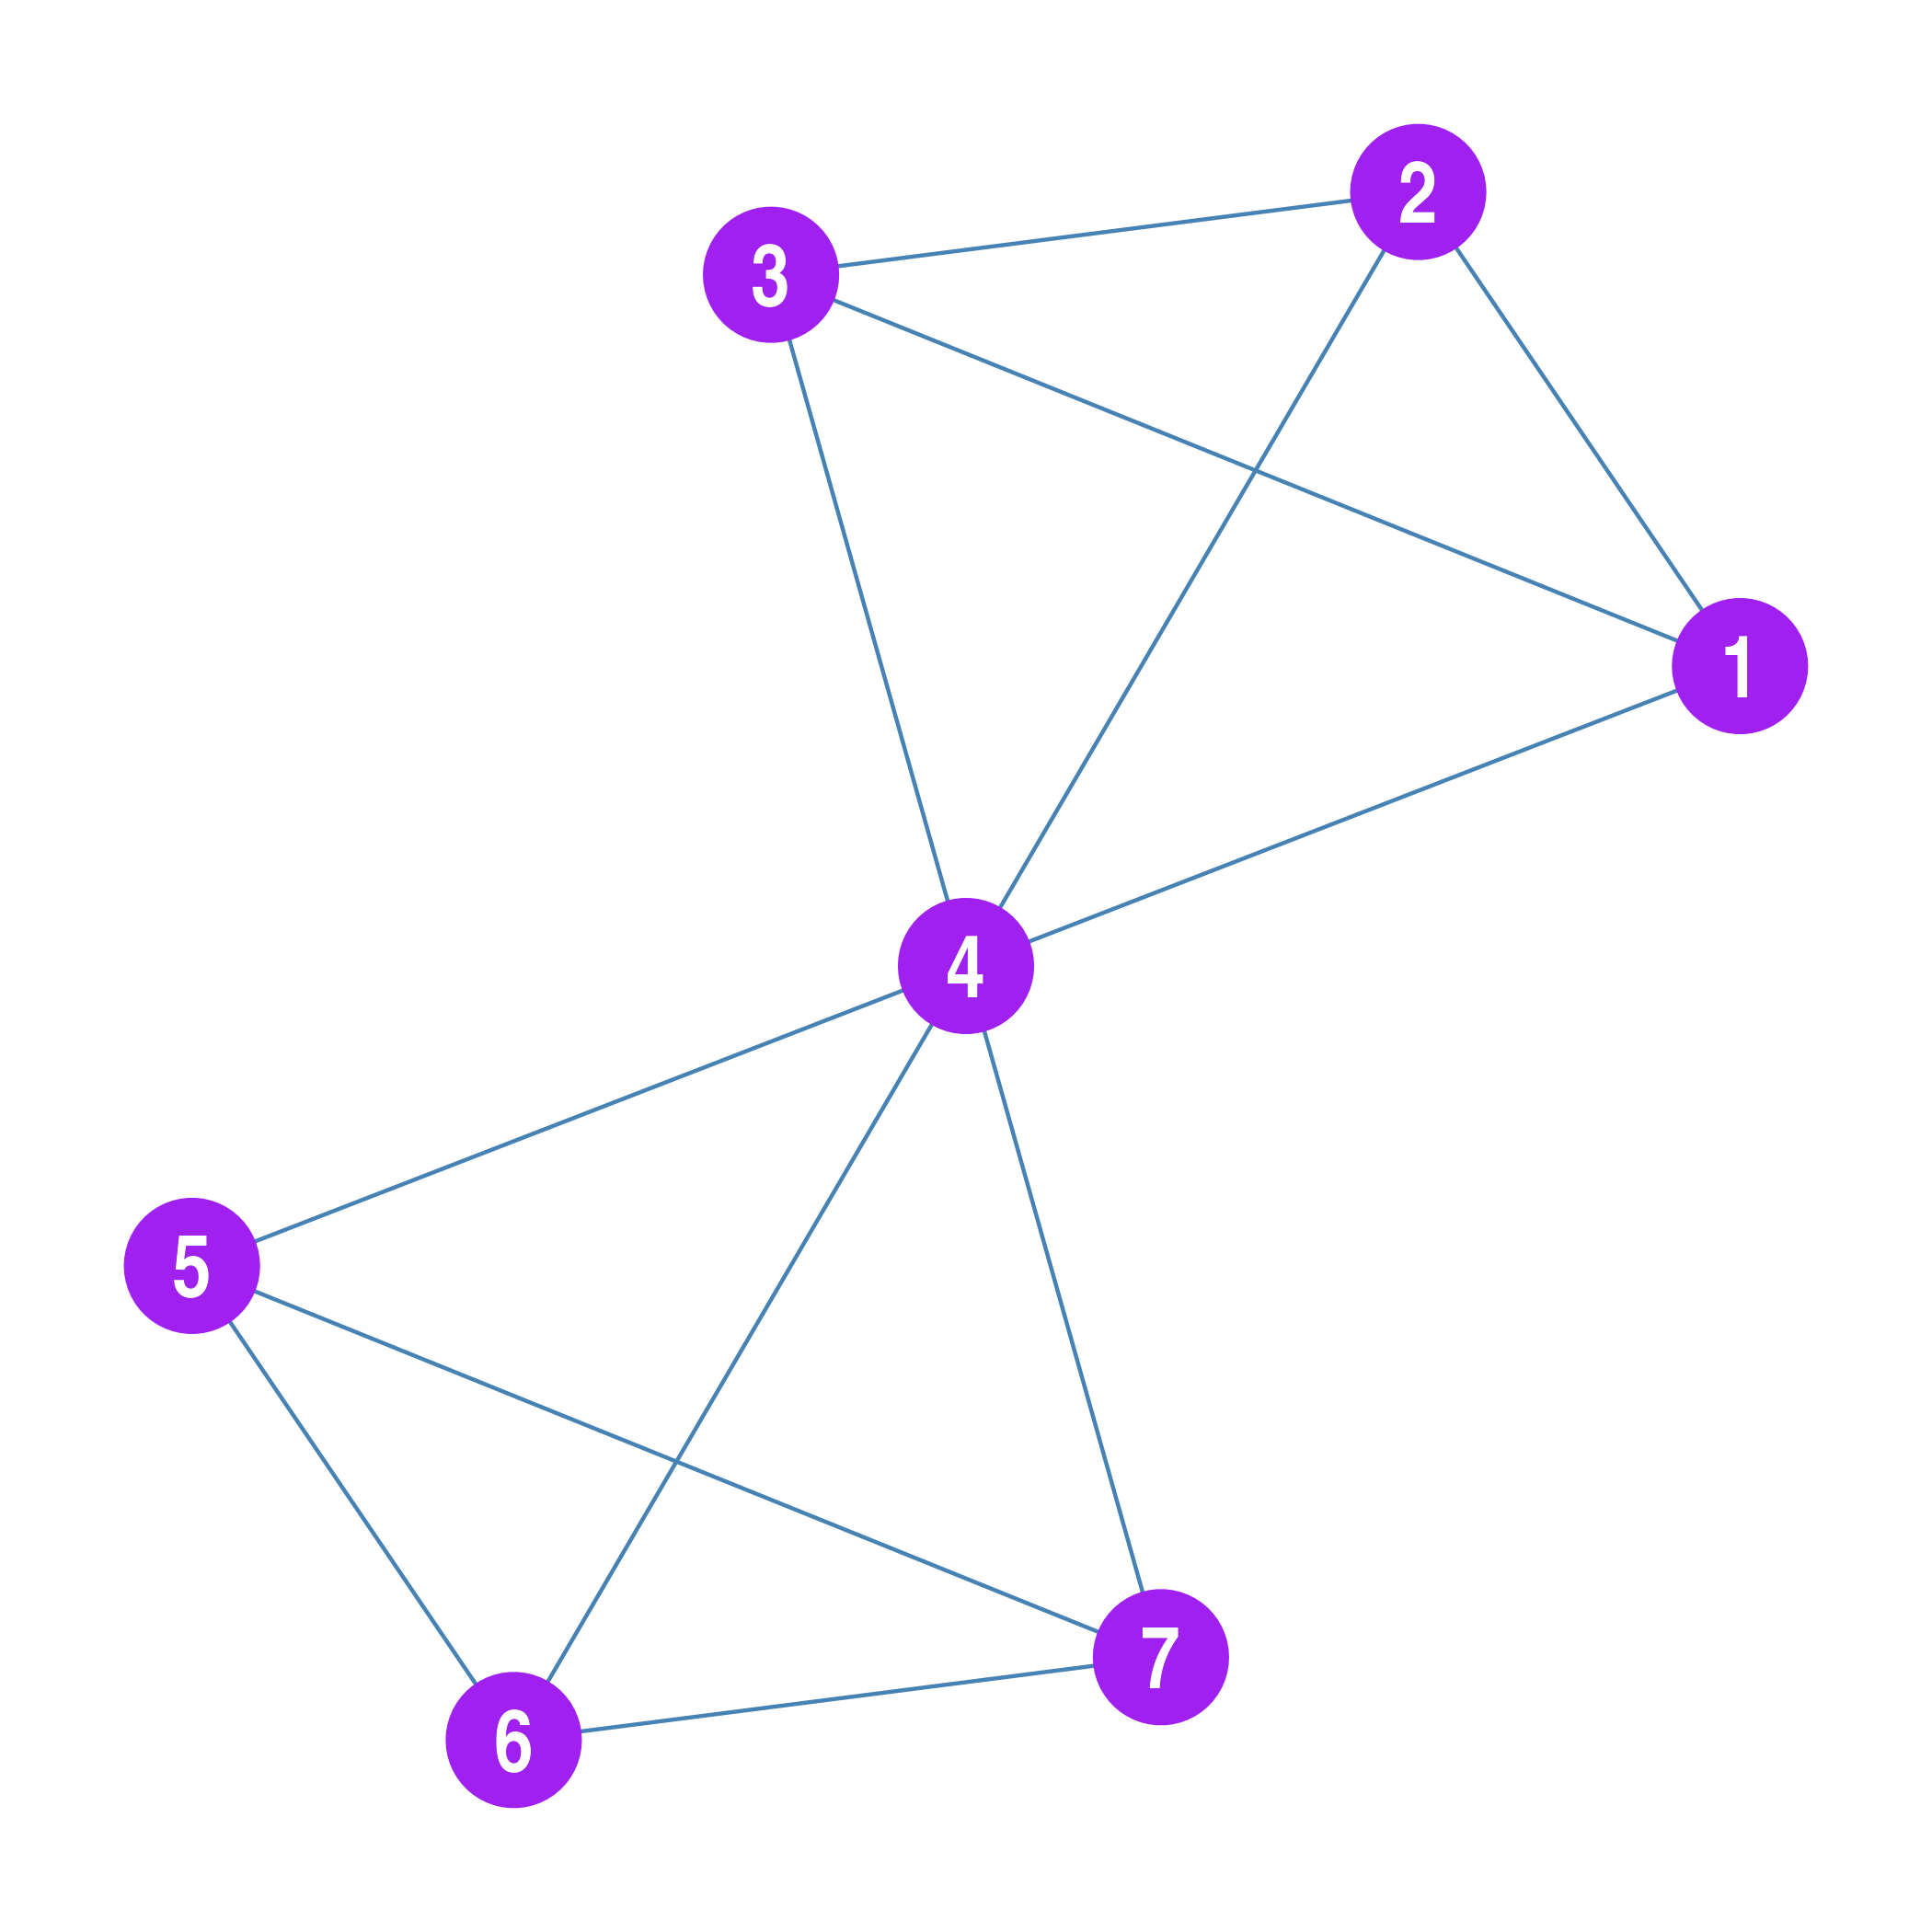
\includegraphics[width=1.0\textwidth]{Plots/sf4.png}
            \caption{Structural Fold (4-Clique)}
            \label{fig:sf4}
    \end{subfigure} 
    \begin{subfigure}[b]{0.23\textwidth}
        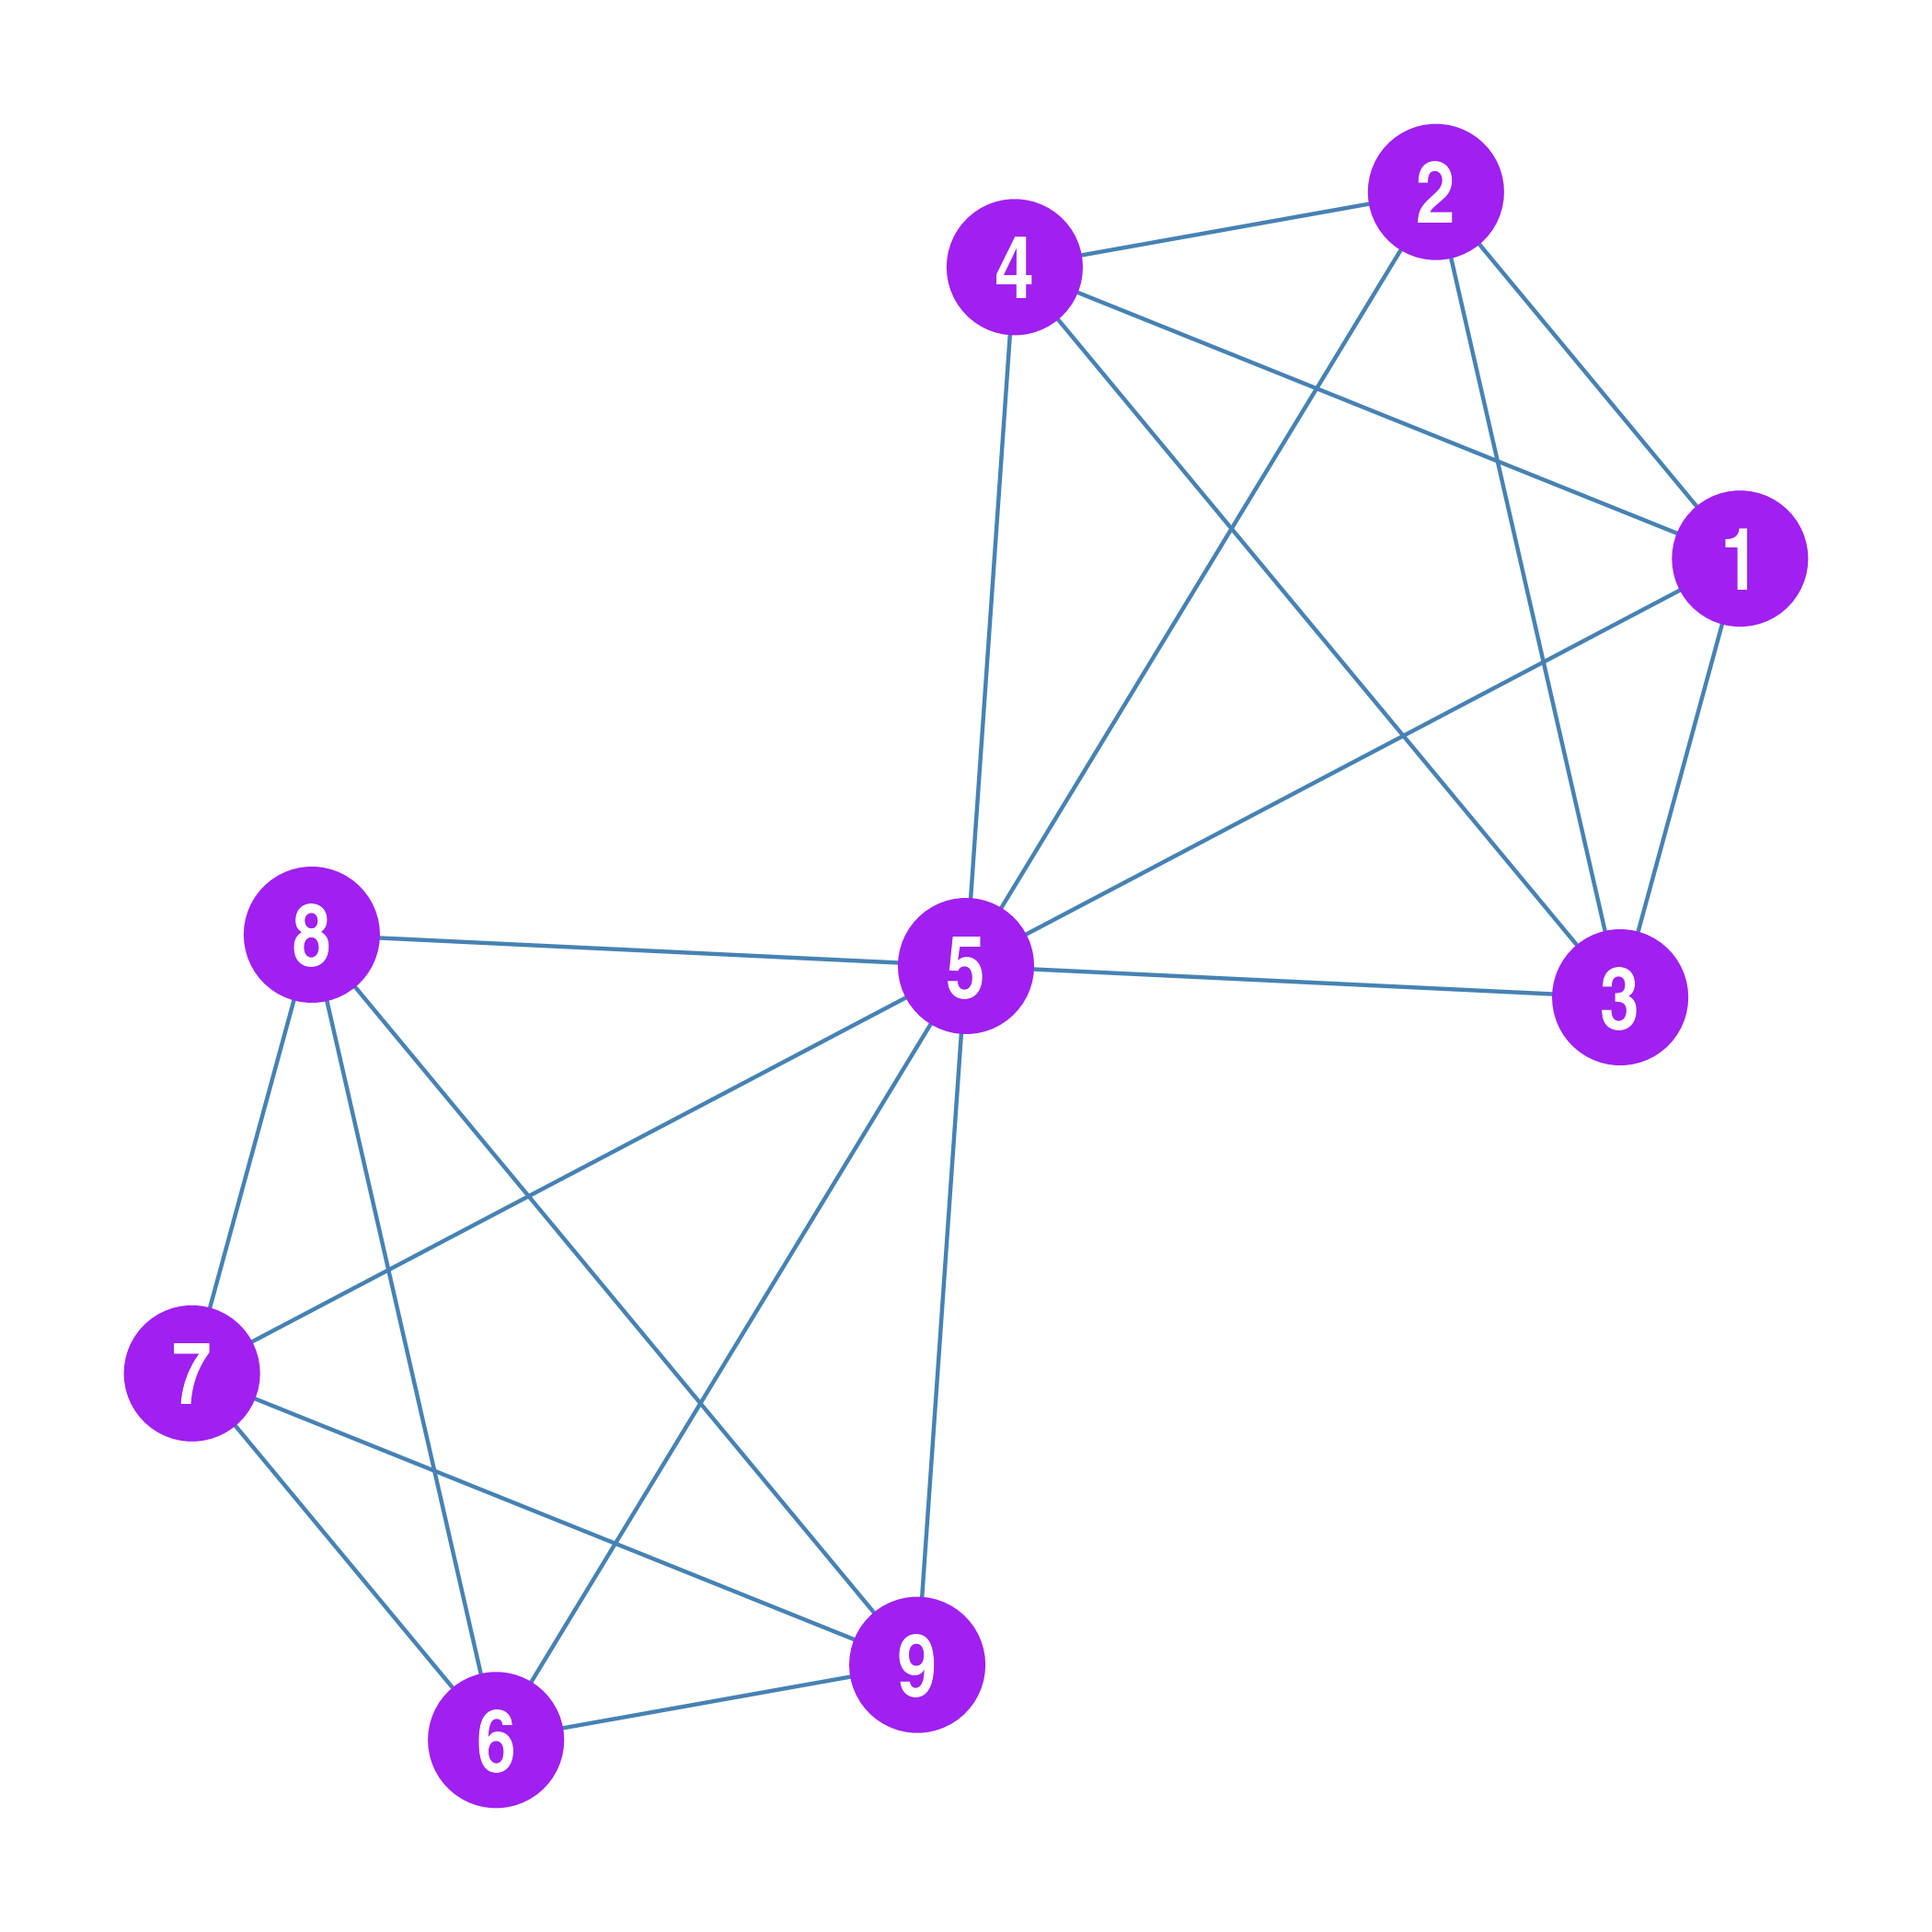
\includegraphics[width=1.0\textwidth]{Plots/sf5.png}
            \caption{Structural Fold (5-Clique)}
            \label{fig:sf5}
    \end{subfigure} 
    \begin{subfigure}[b]{0.23\textwidth}
        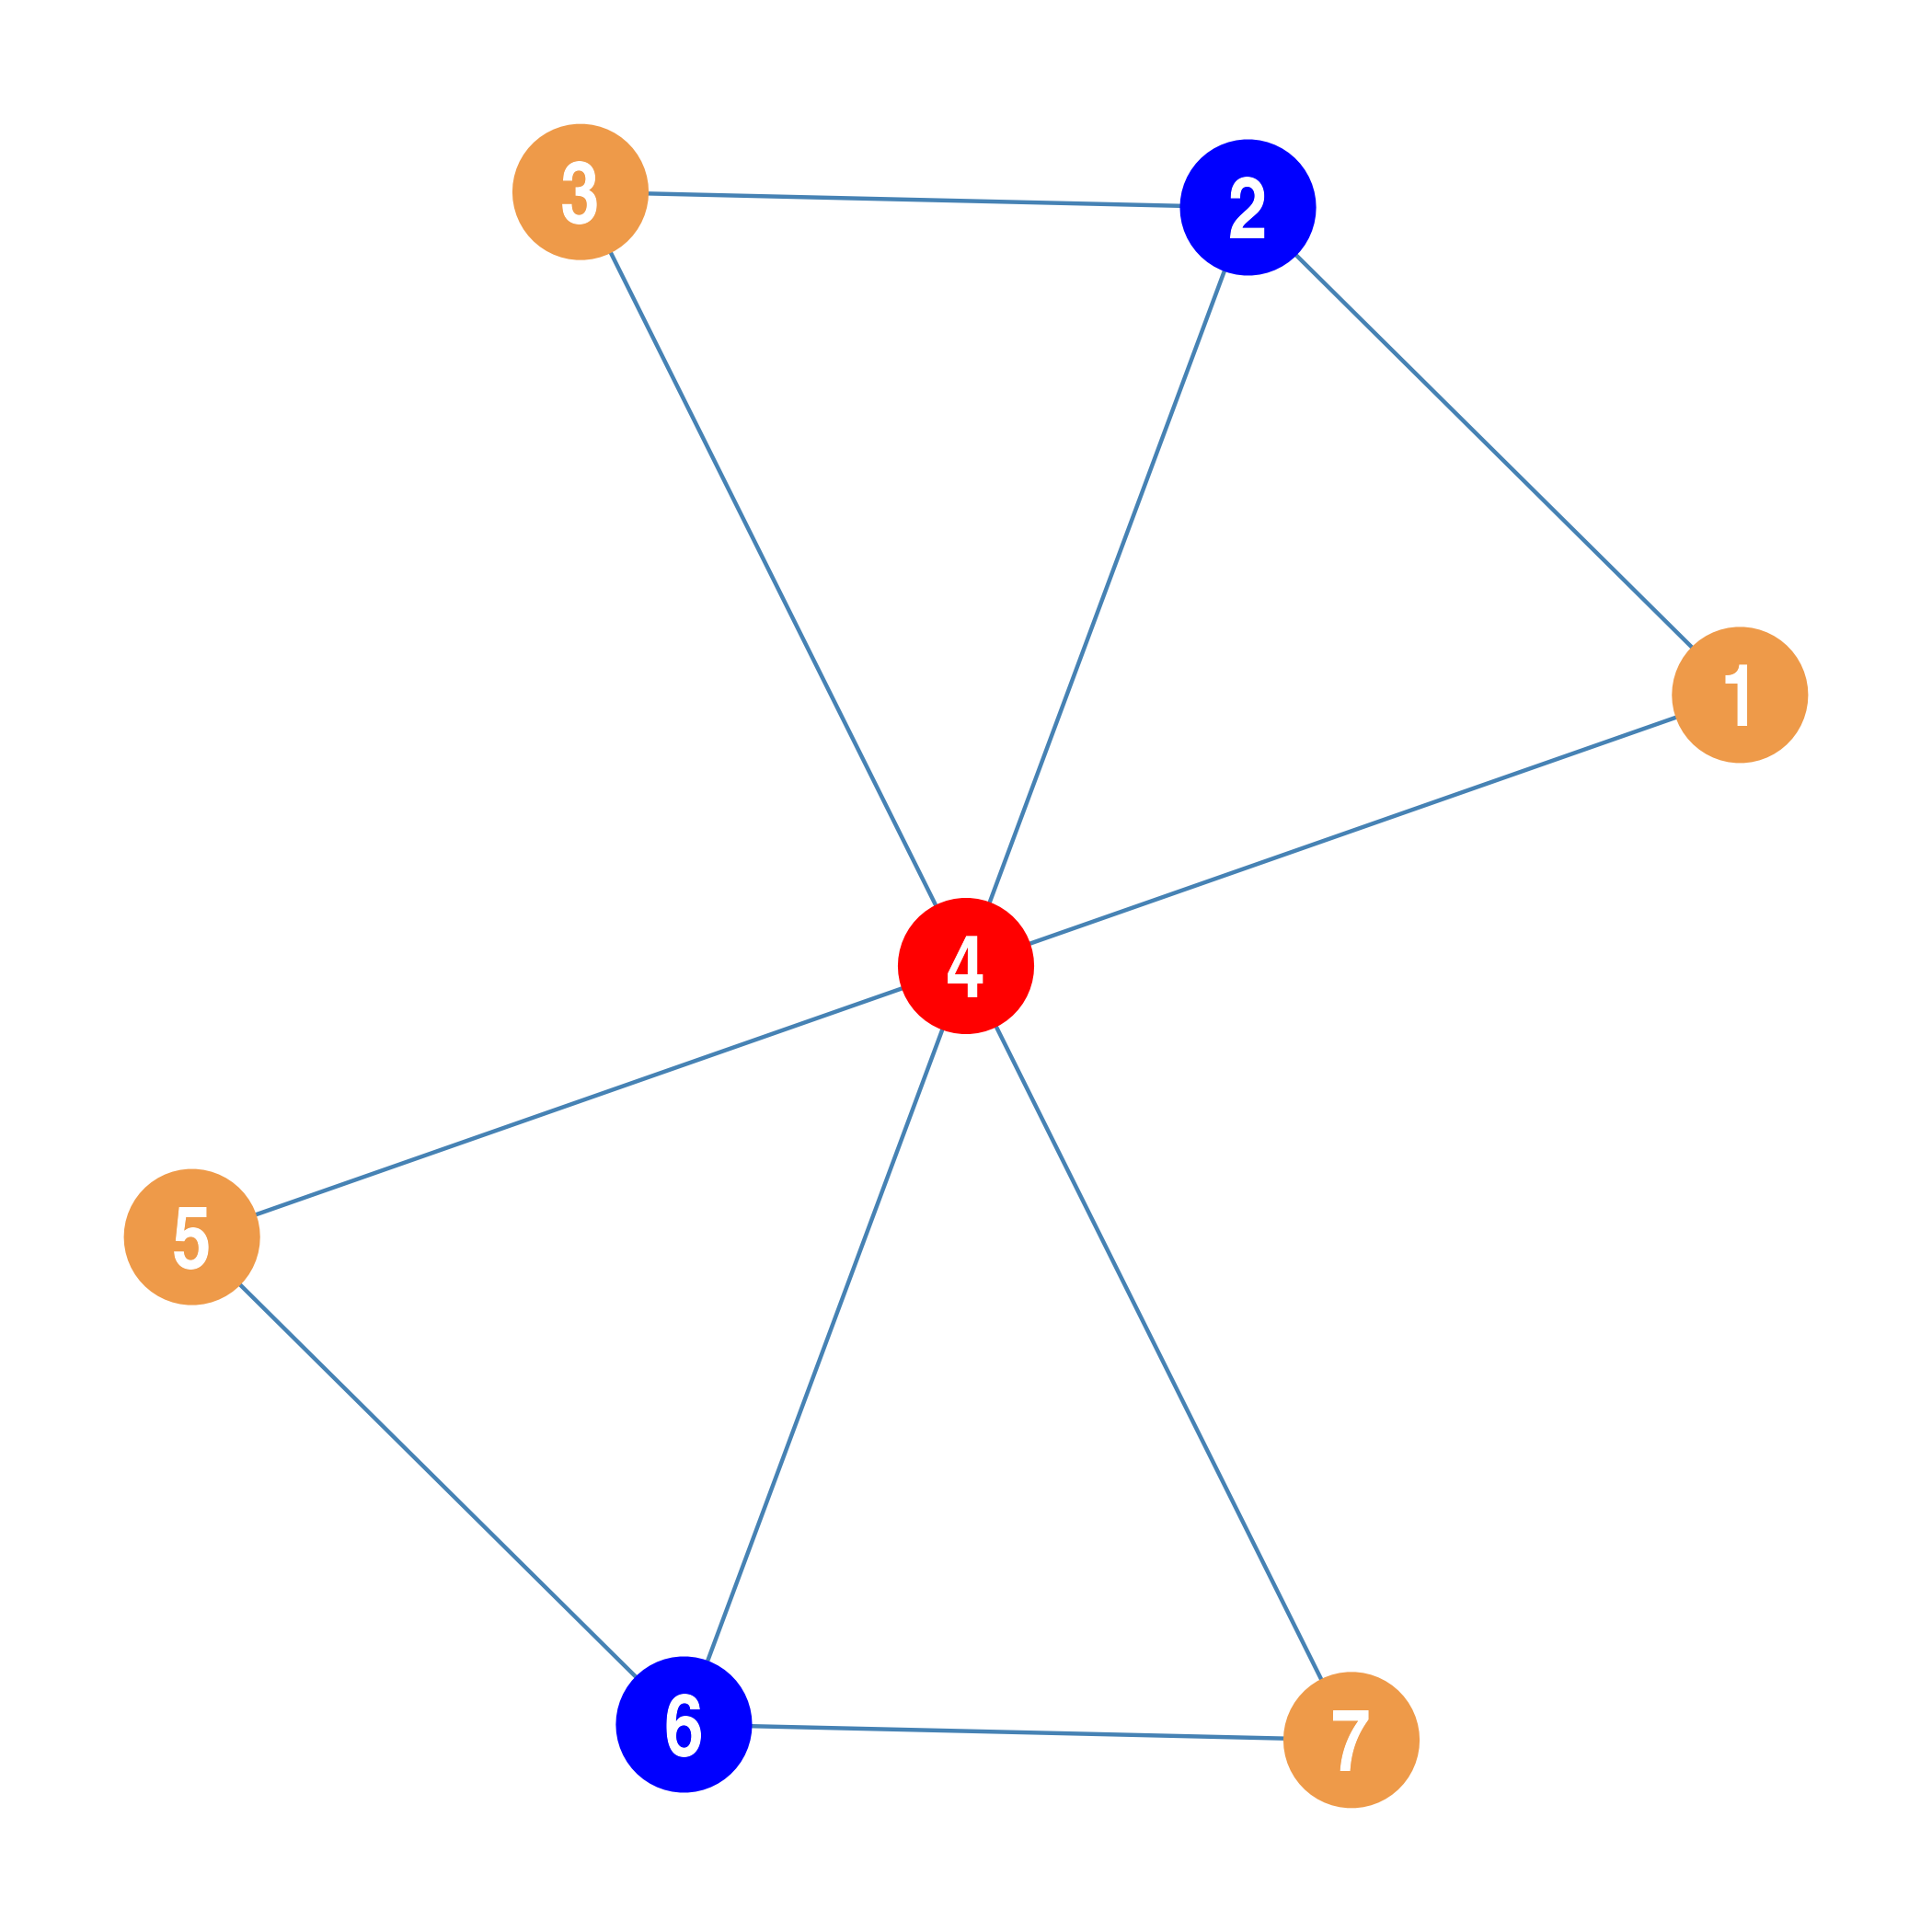
\includegraphics[width=1.0\textwidth]{Plots/two-connected.png}
            \caption{Two-Connected}
            \label{fig:twoconnected}
    \end{subfigure} 
    \begin{subfigure}[b]{0.23\textwidth}
        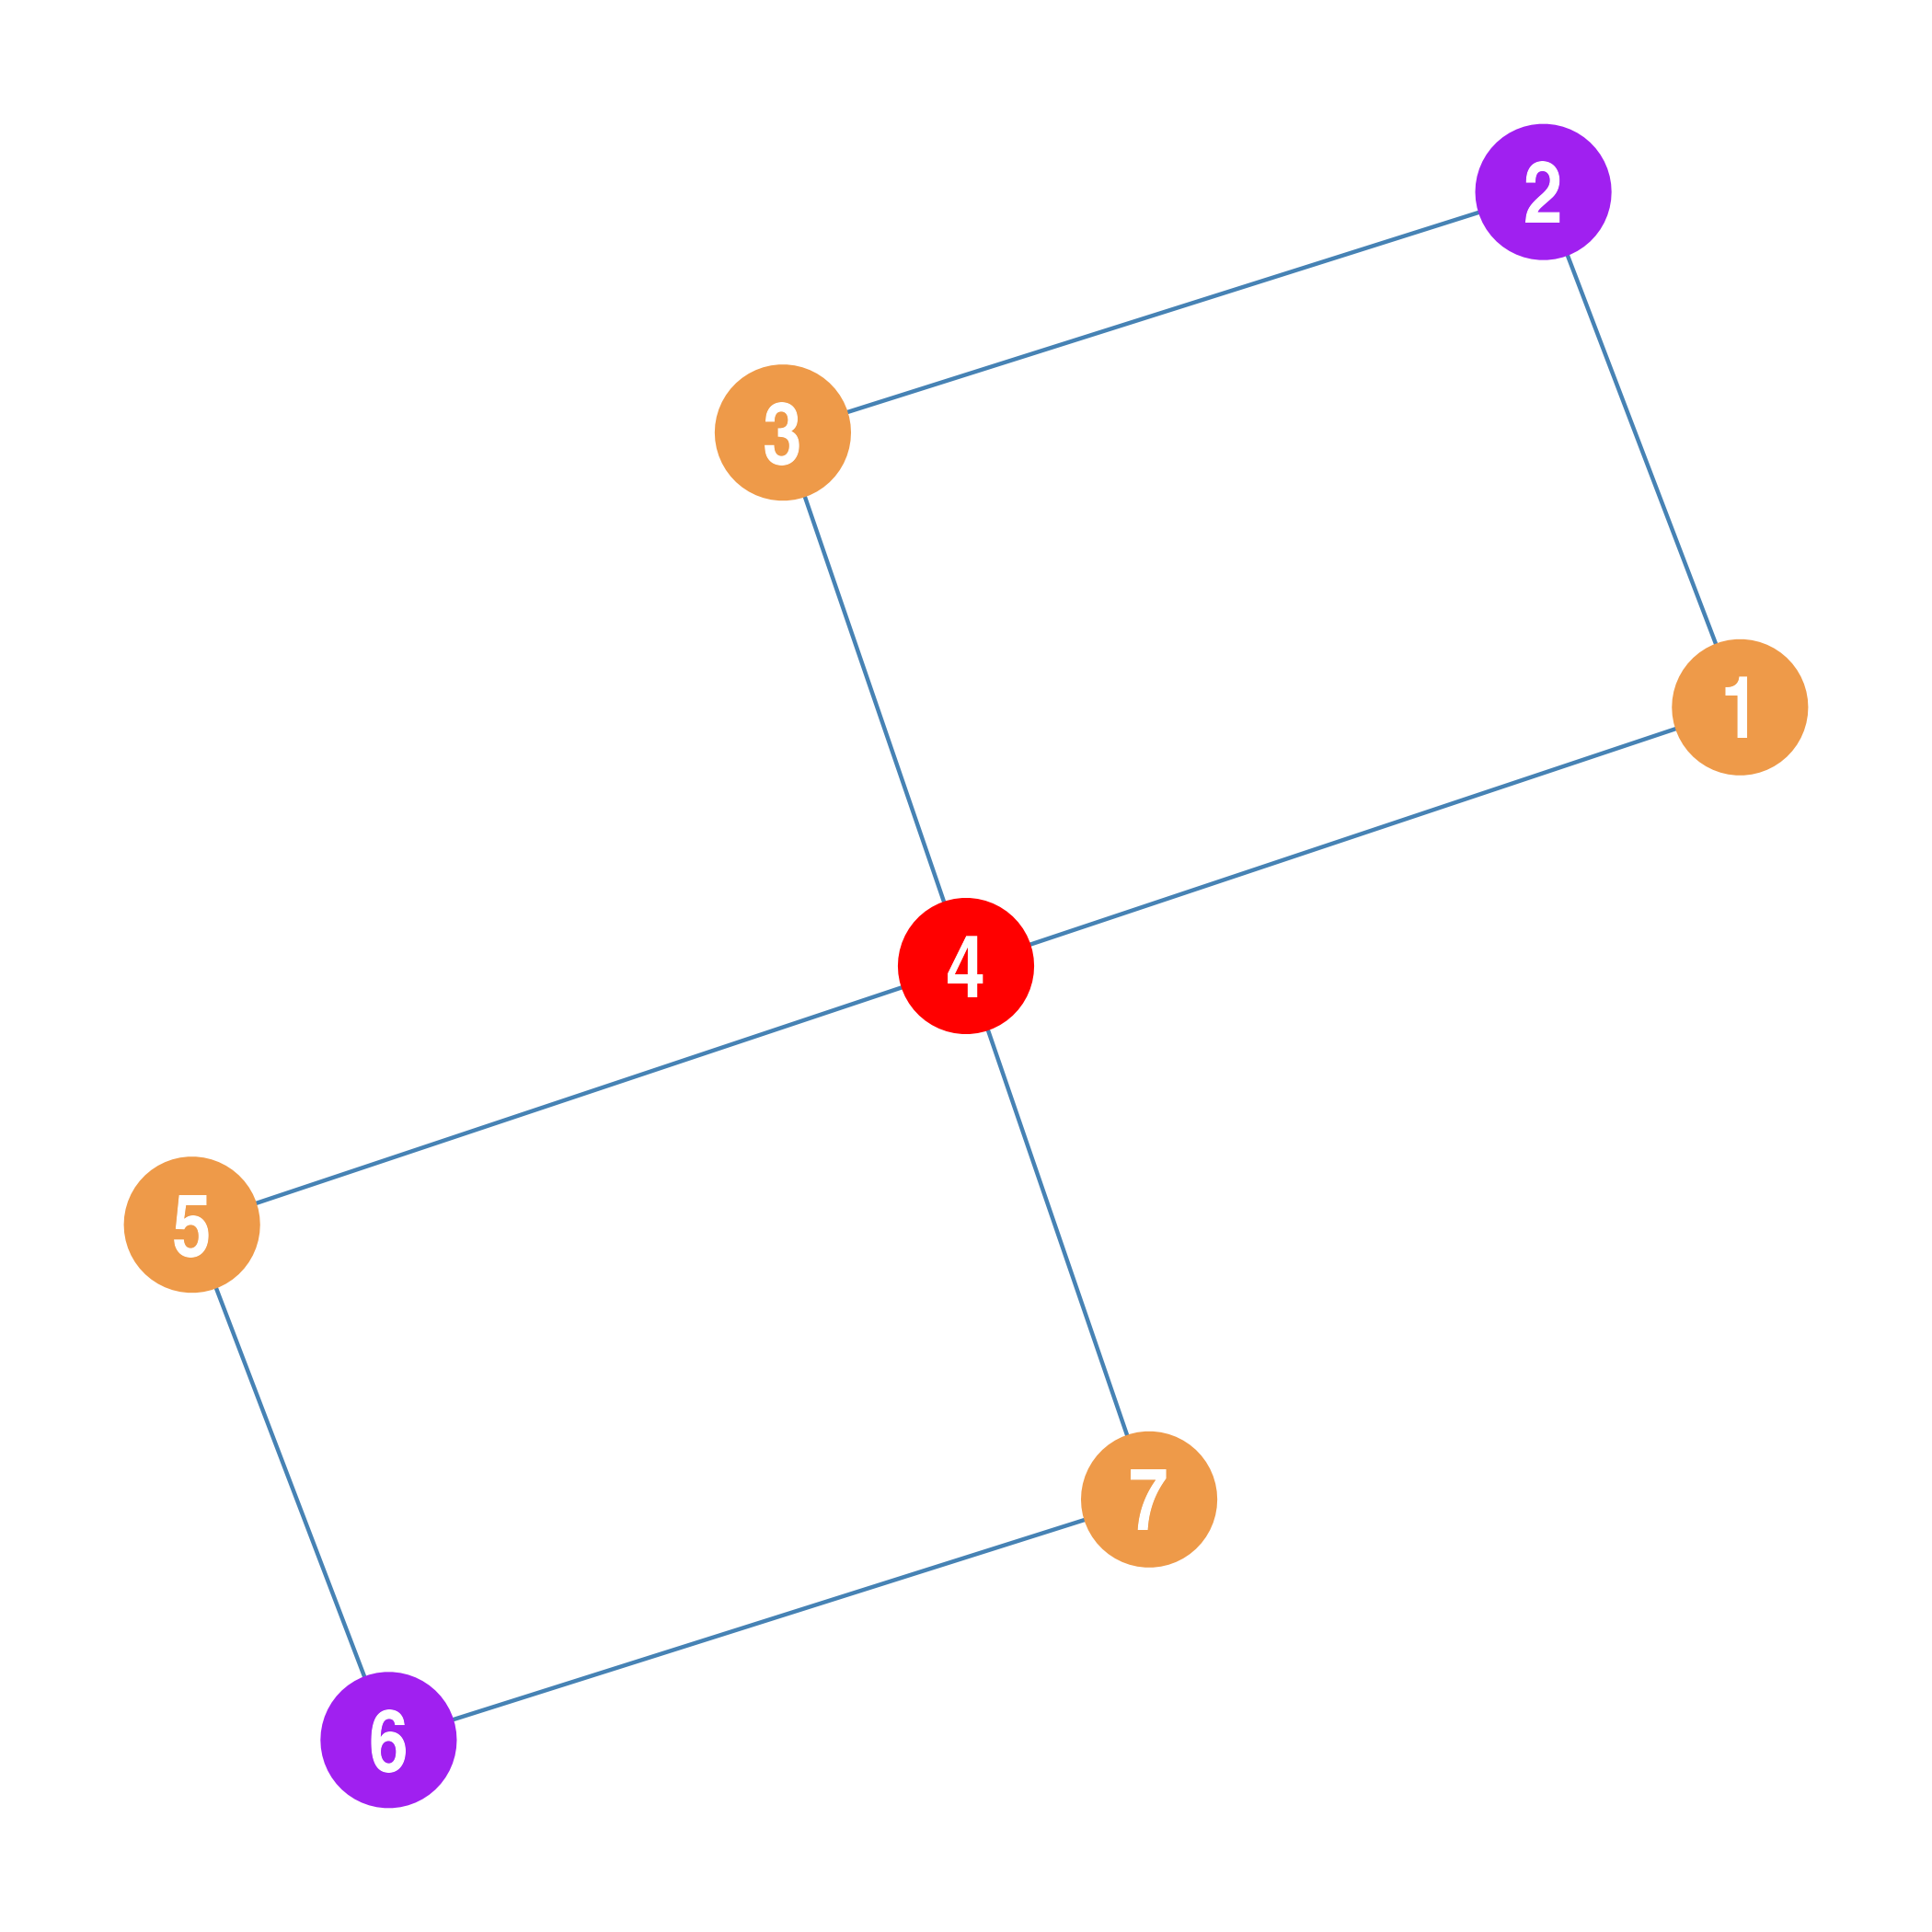
\includegraphics[width=1.0\textwidth]{Plots/circle-weld.png}
            \caption{Circle Weld}
            \label{fig:circleweld}
    \end{subfigure} 
    \begin{subfigure}[b]{0.23\textwidth}
        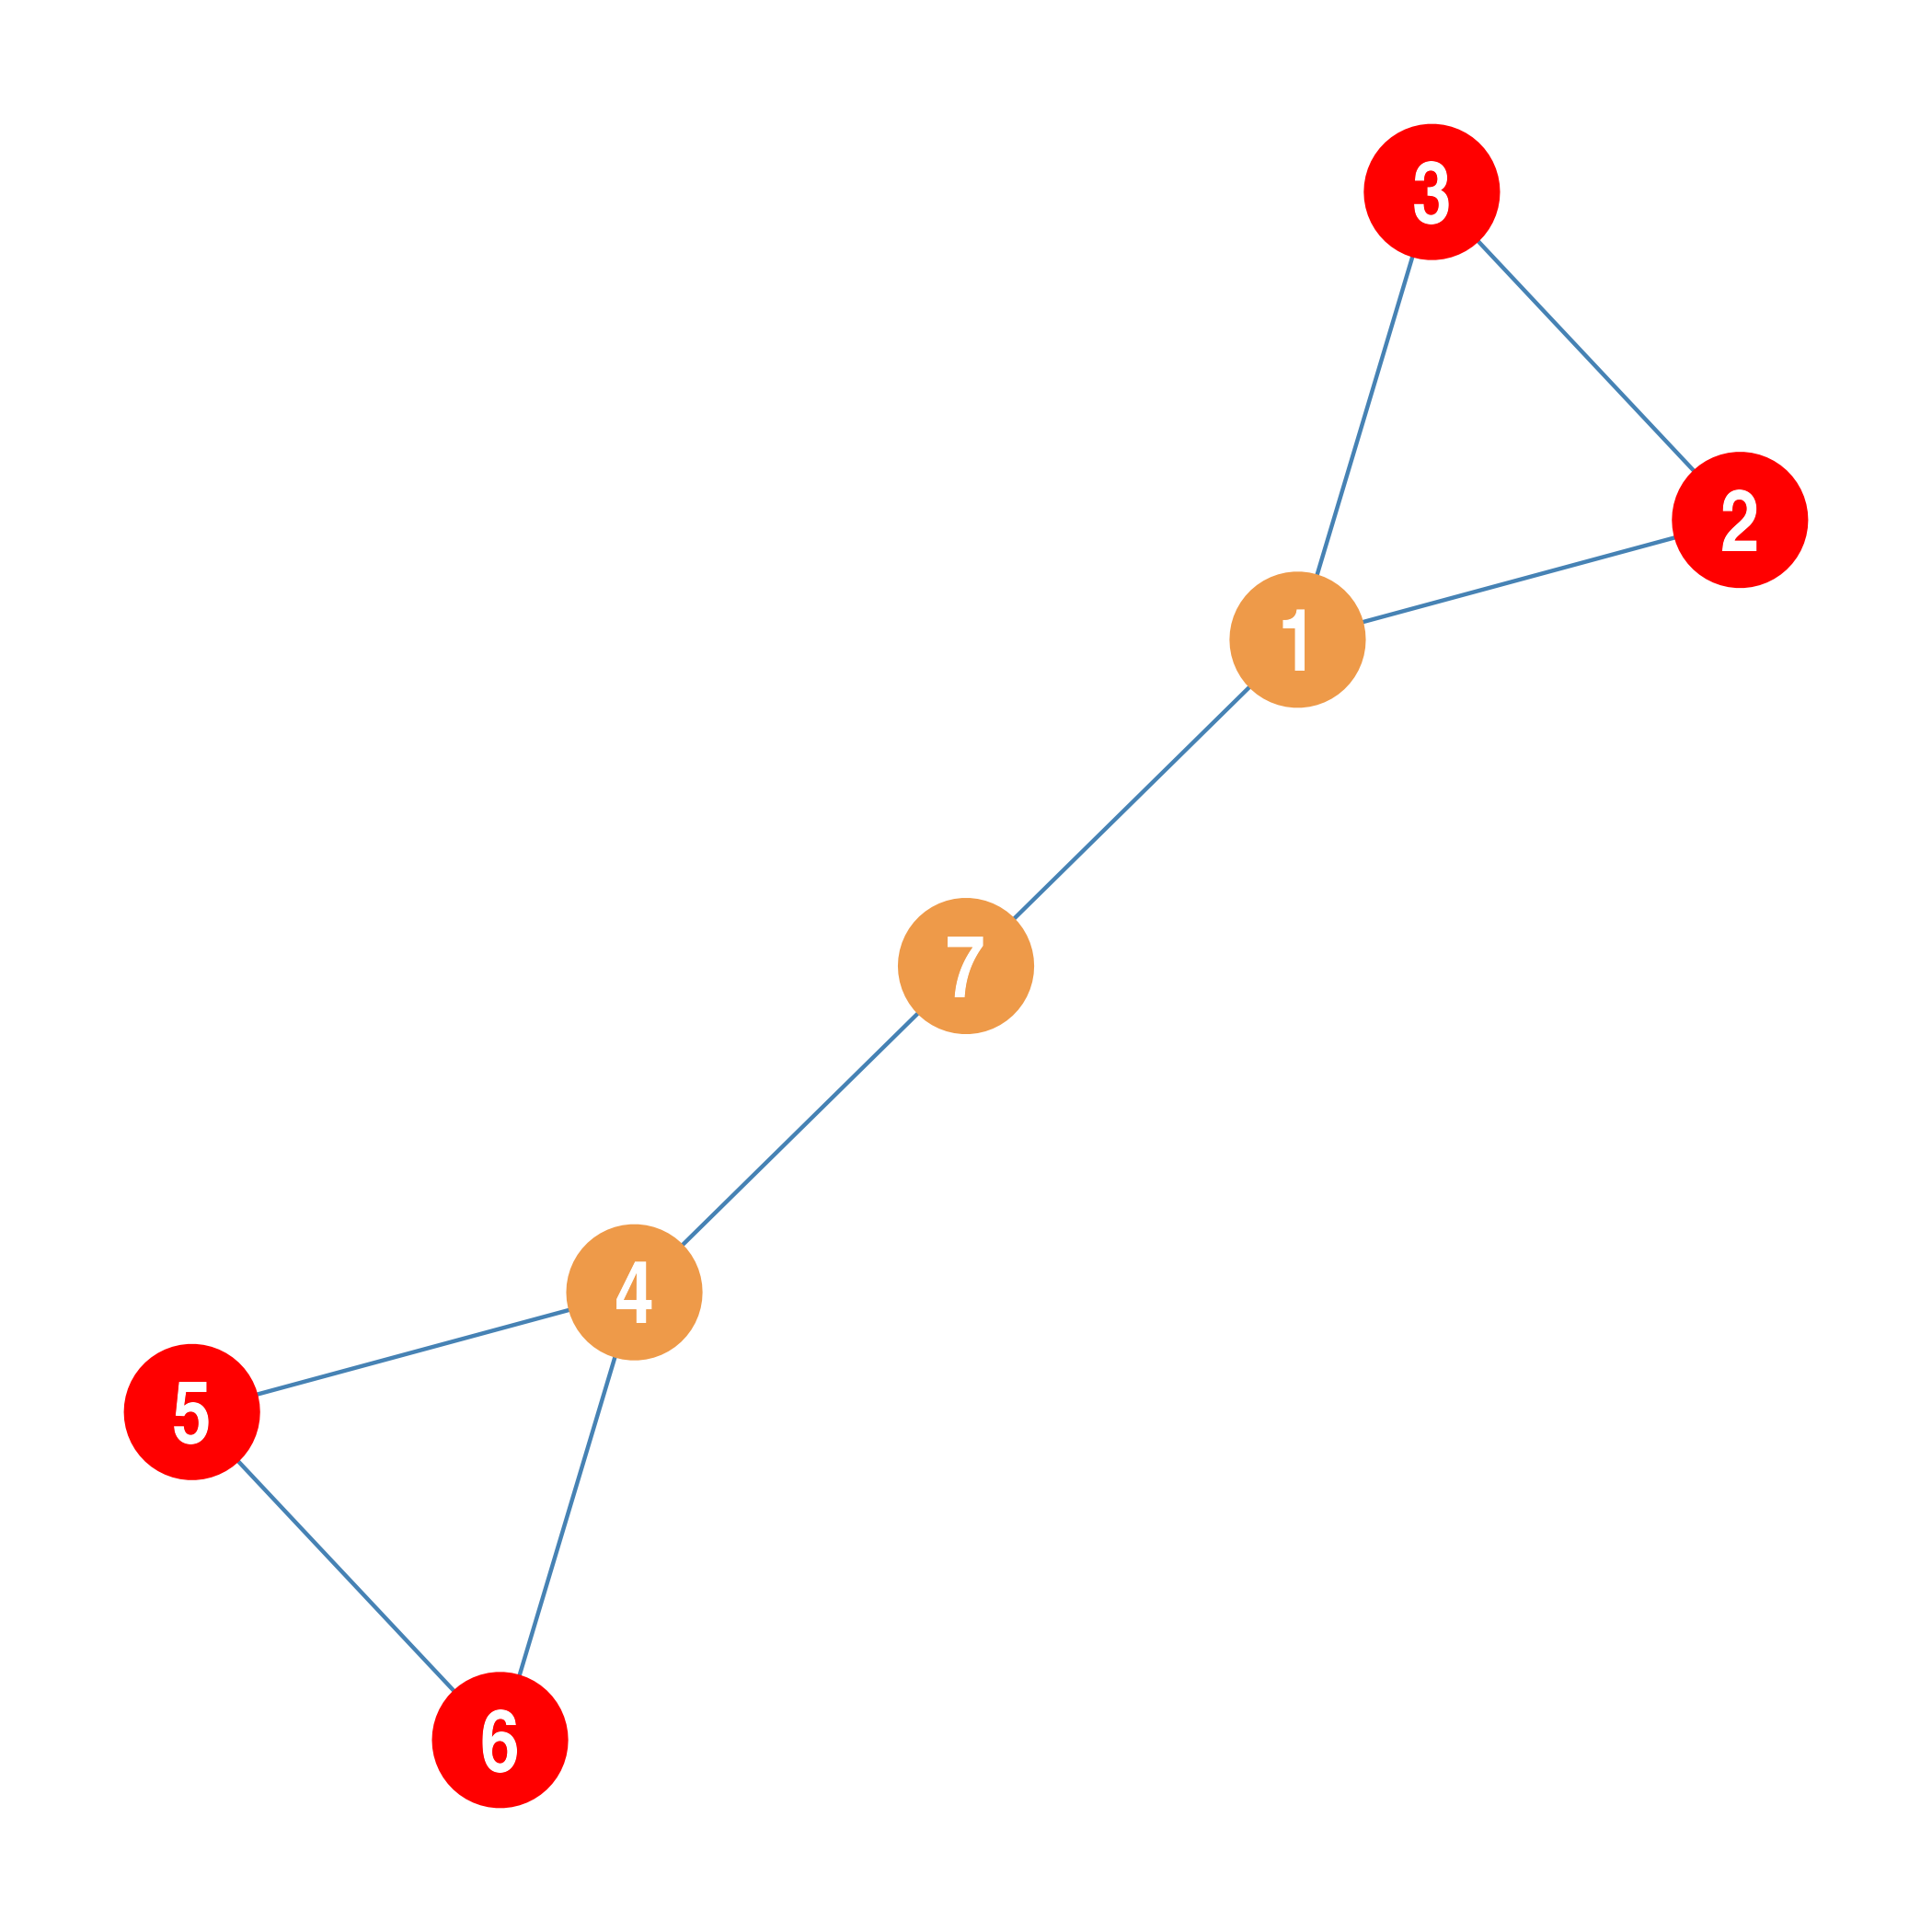
\includegraphics[width=1.0\textwidth]{Plots/broker3.png}
            \caption{Brokerage Mediated (3-Cliques)}
            \label{fig:broker3}
    \end{subfigure} 
    \label{fig:struct-fold}
    \begin{subfigure}[b]{0.23\textwidth}
        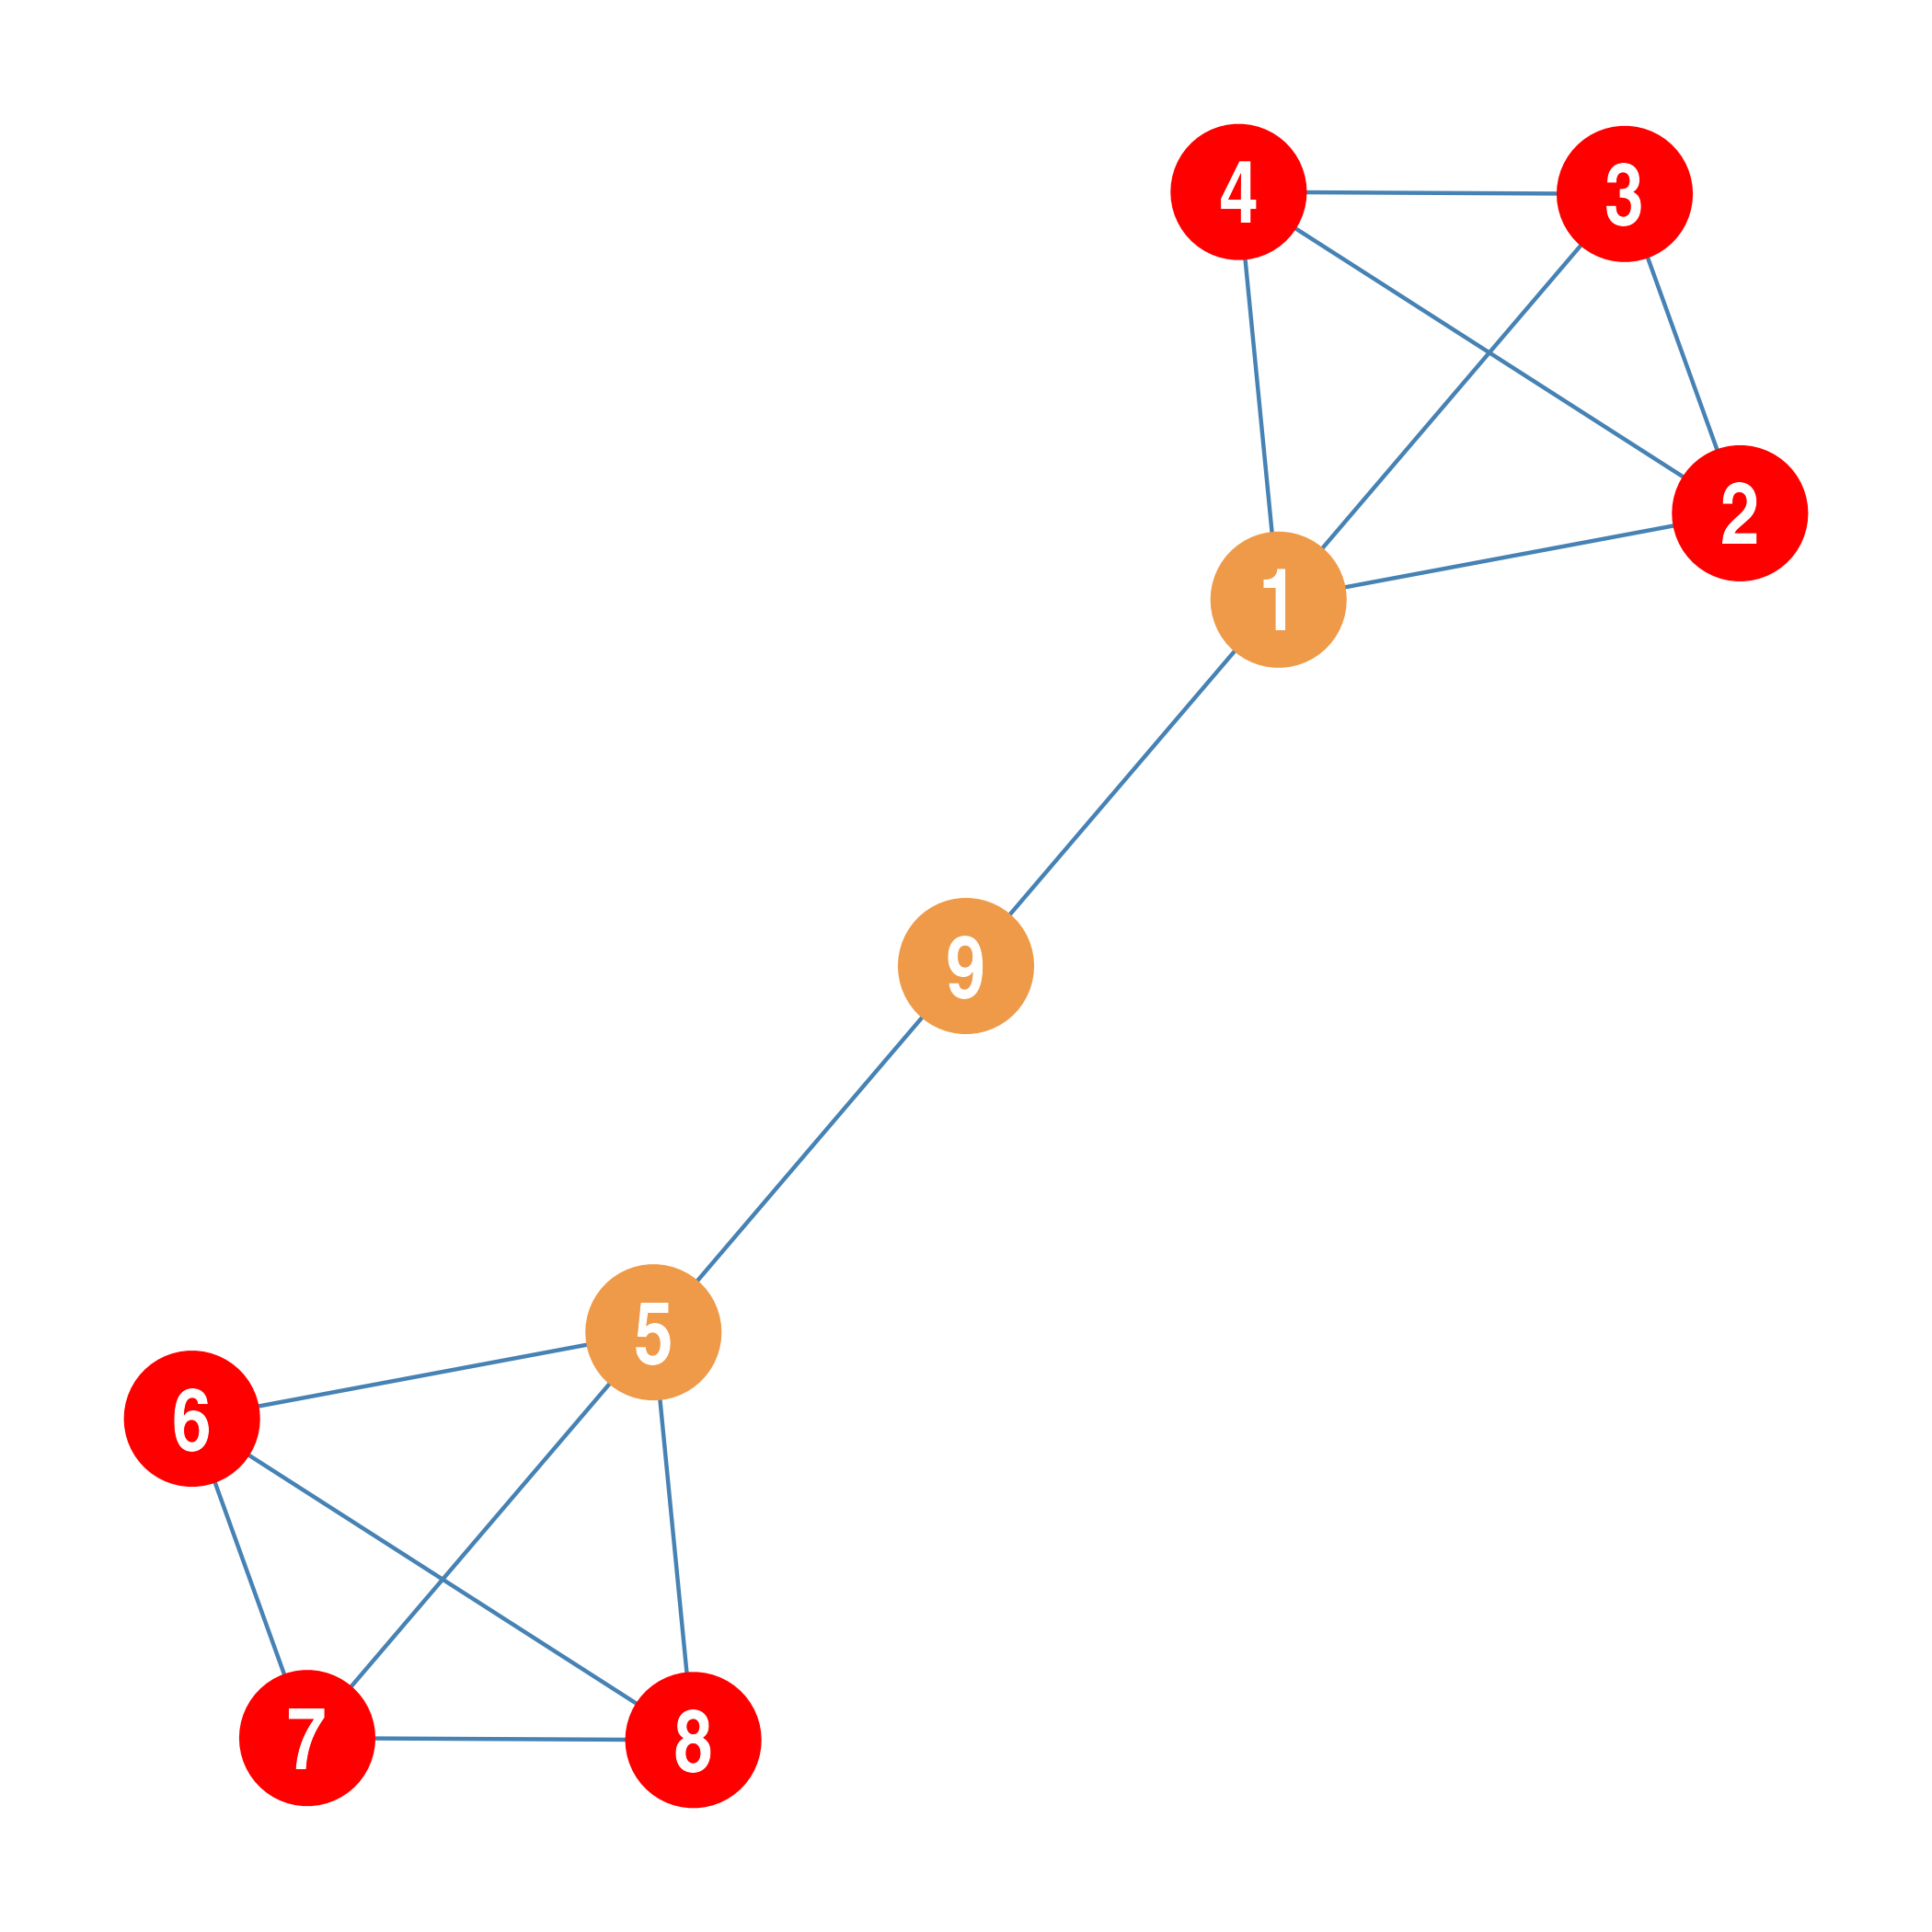
\includegraphics[width=1.0\textwidth]{Plots/broker4.png}
            \caption{Brokerage Mediated (4-Cliques)}
            \label{fig:broker4}
    \end{subfigure} 
    \begin{subfigure}[b]{0.23\textwidth}
        
\includegraphics[width=1.0\textwidth]{Plots/tree-mediator2.png}
            \caption{Tree with 2 Branches, 2 Leaves}
            \label{fig:treemediator2}
    \end{subfigure} 
    \begin{subfigure}[b]{0.23\textwidth}
        
\includegraphics[width=1.0\textwidth]{Plots/tree-mediator3.png}
            \caption{Tree with 2 Branches, 3 Leaves}
            \label{fig:treemediator3}
    \end{subfigure}
    \begin{subfigure}[b]{0.23\textwidth}
        
\includegraphics[width=1.0\textwidth]{Plots/tree-mediator2-long.png}
            \caption{Tree with 2 Branches, 2 Leaves, 1 Long Tie}
            \label{fig:treemediatorlong2}
    \end{subfigure}
    \begin{subfigure}[b]{0.23\textwidth}
        
\includegraphics[width=1.0\textwidth]{Plots/tree-mediator3-long.png}
            \caption{Tree with 2 Branches, 3 Leaves, 1 Long Tie}
            \label{fig:treemediatorlong3}
    \end{subfigure}
    \caption{Comparison of betweenness brokerage and a structural folds Distinction Centrality in toy graphs. Nodes with the highest distinction are shown in red, nodes with positive distinction are shown in blue, nodes with negative distinction are shown in tan, and nodes with distinction close to zero are shown in purple.}
\end{figure}

%brokerage centrality scores
\input{Tabs/Figure4}

\textit{Model (c)} presents a graph that is 2-connected in the absence of node 1. Each subgraph is one connection short of forming complete subgraphs in the absence of Node 1. Compared to the structural fold, connections 3-2 and 6-7 have been removed. Measurement results are in Table 3. Of the demonstrative networks here, this is the one that most approximates a three-tiered ordered hierarchy. The resulting scalar-adjusted distinction measures well reflect this stratification, with Node 1 retaining its position, Nodes 4 and 5 occupying the middle, and Nodes 2, 3, 6, and 7 falling to the bottom. 

\textit{Model (d)} is the same 2-connected graph with the addition of a long tie connecting nodes 2 and 7. This long tie stratifies the network even more than in Model (c), bringing Nodes 2 and 7 quite close to 4 and 5. The formation of the long tie served to bolster the individual distinction of 2 and 7 more than the formation of the tie that would create the completely connected subgraphs, as in Model (b). In fact, all nodes except 3 and 6 have greater distinction in this case. This reflects the positional idea that distinction is a matter of stratification, and cohesion is at odds with creating stratification. While the status of Nodes 2 and 7 actually increases beyond that of Nodes 4 and 5 due to the long tie, the constraint also increases as they are now both further constrained by the influence of Node 1, their mutual neighbor.  




\subsubsection{Kite Graphs and Eigenvector Normalization}


%%% FIGURE 5 KITE GRAPHS
\begin{figure}
    \captionsetup[subfigure]{font=footnotesize,labelfont=footnotesize}
    \centering
    \begin{subfigure}[b]{0.23\textwidth}
        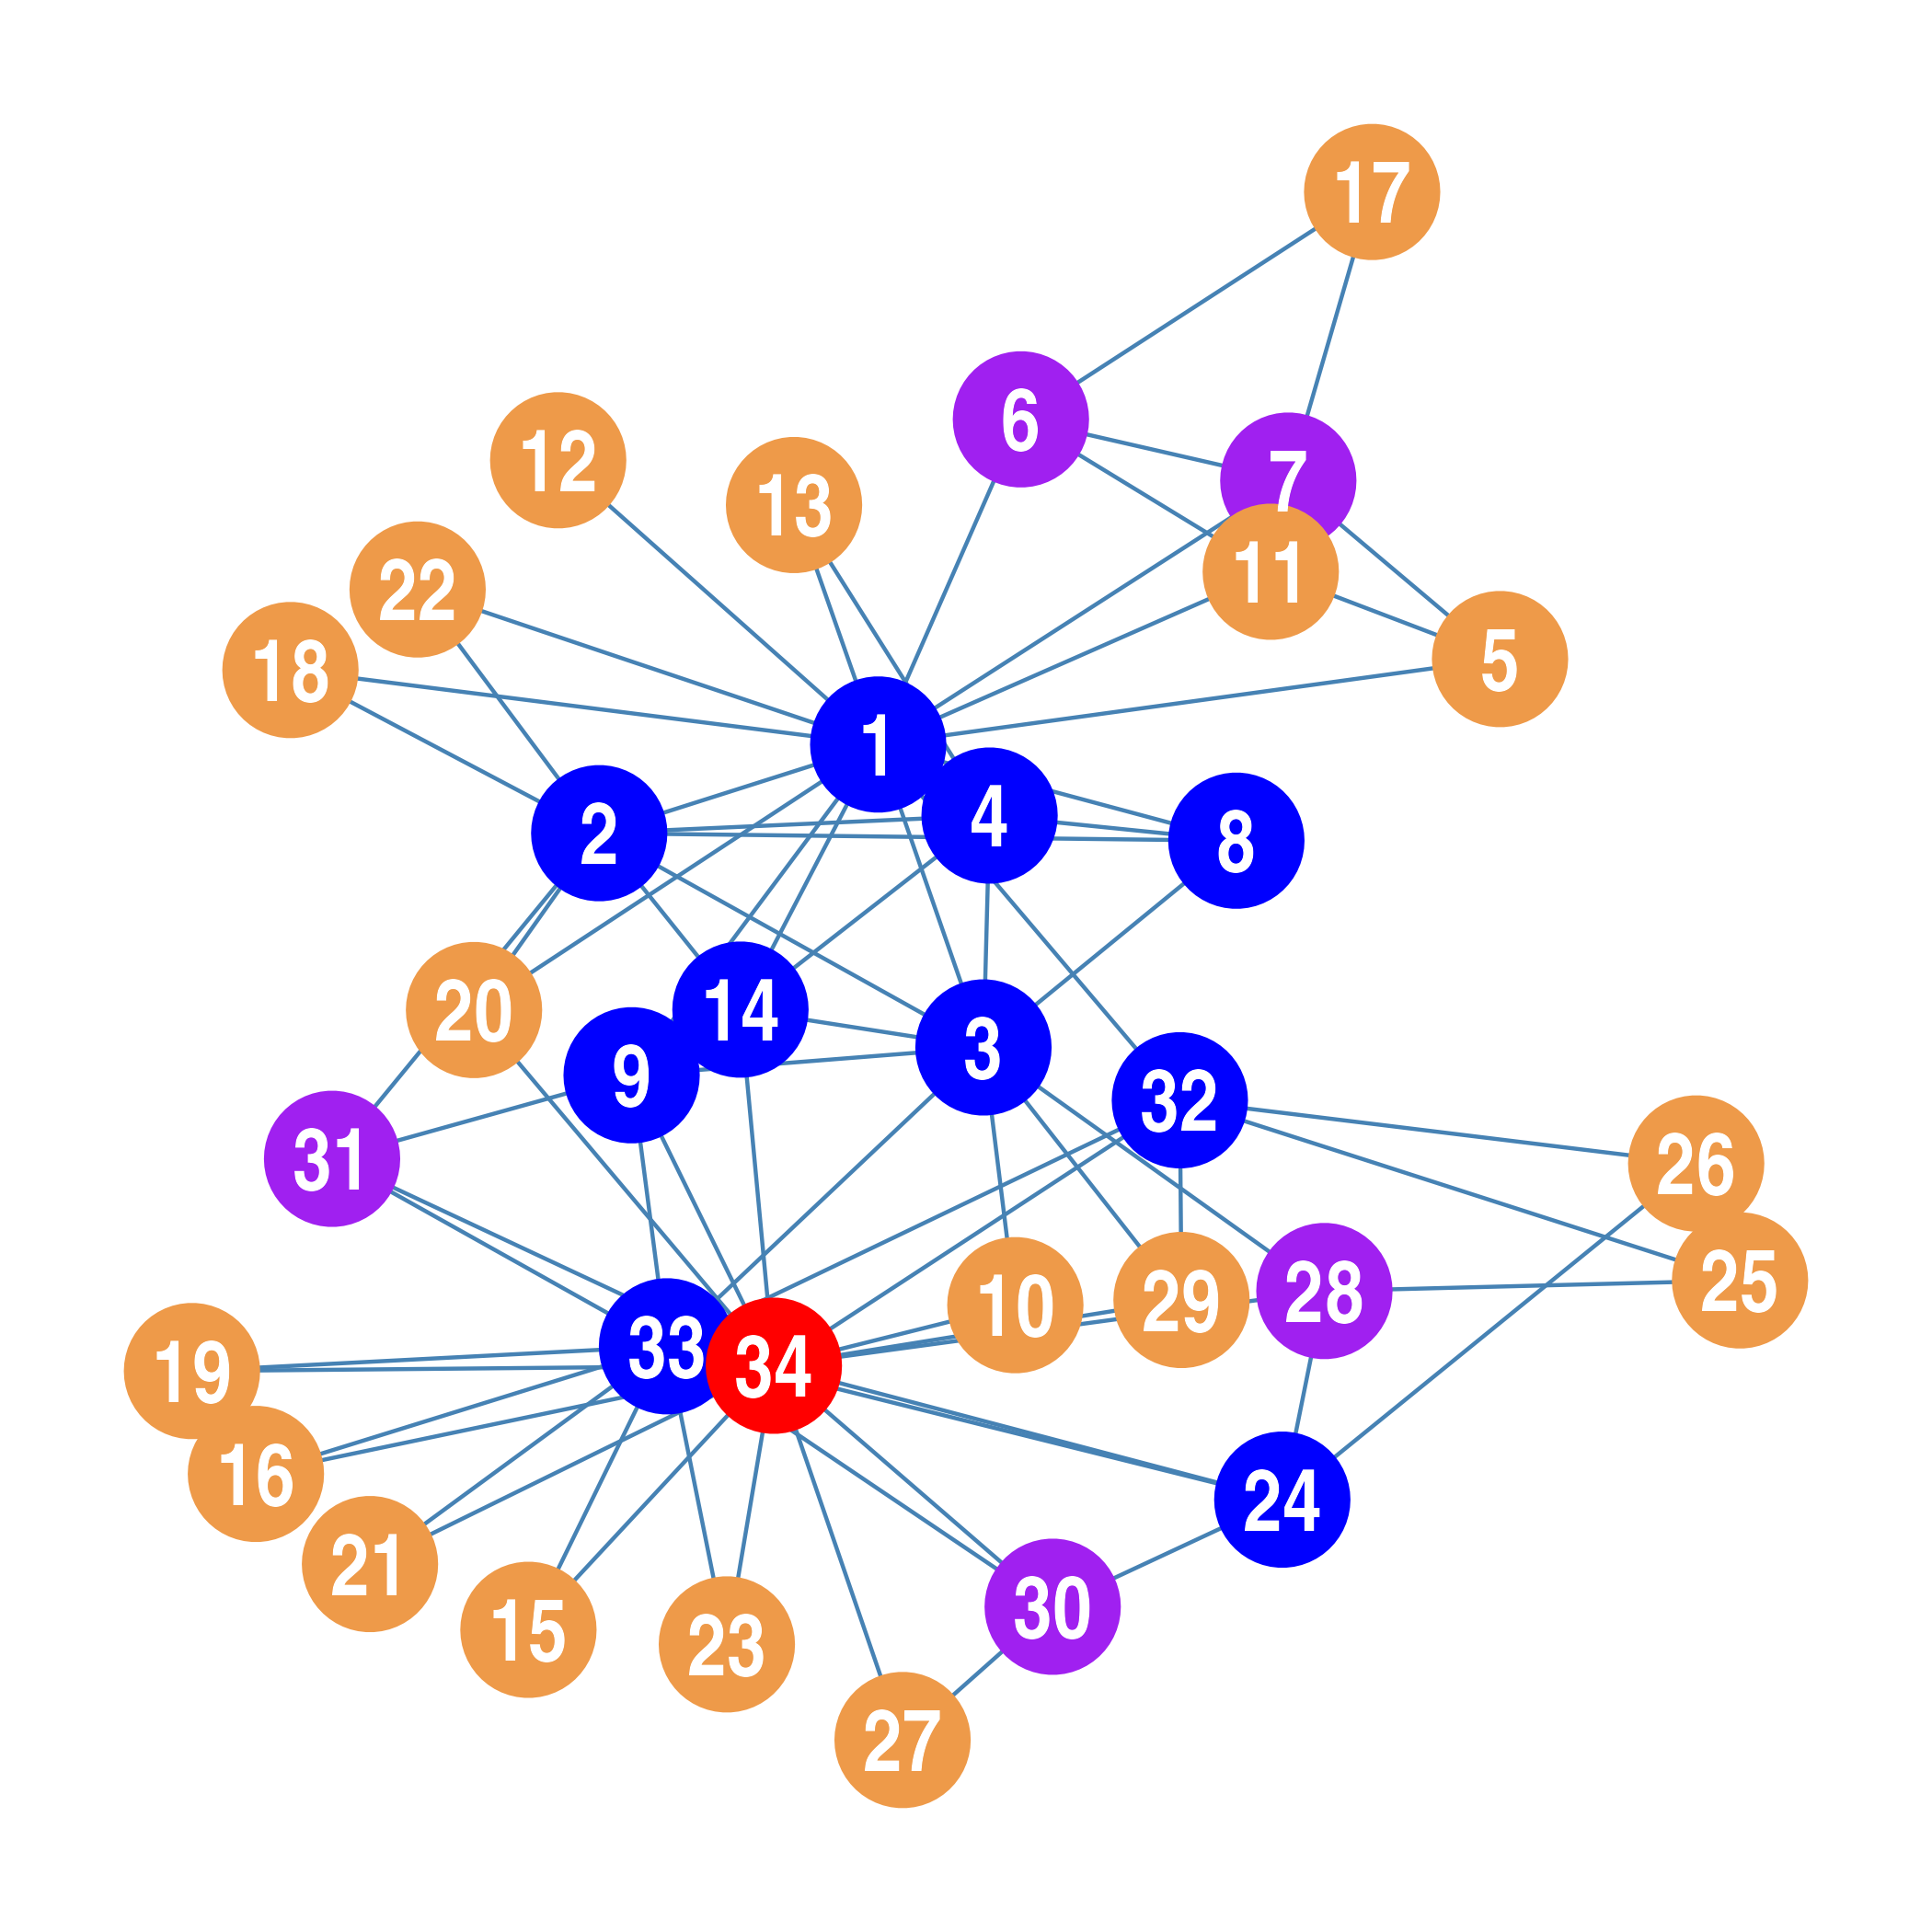
\includegraphics[width=1.0\textwidth]{Plots/kite.png}
            \caption{Three-Clique/Wheel}
            \label{fig:kite-wheel}
    \end{subfigure}
    \begin{subfigure}[b]{0.23\textwidth}
        
\includegraphics[width=1.0\textwidth]{Plots/circle-edge.png}
            \caption{Six-Node Circle}
            \label{fig:circle-edge}
    \end{subfigure} 
    \begin{subfigure}[b]{0.23\textwidth}
        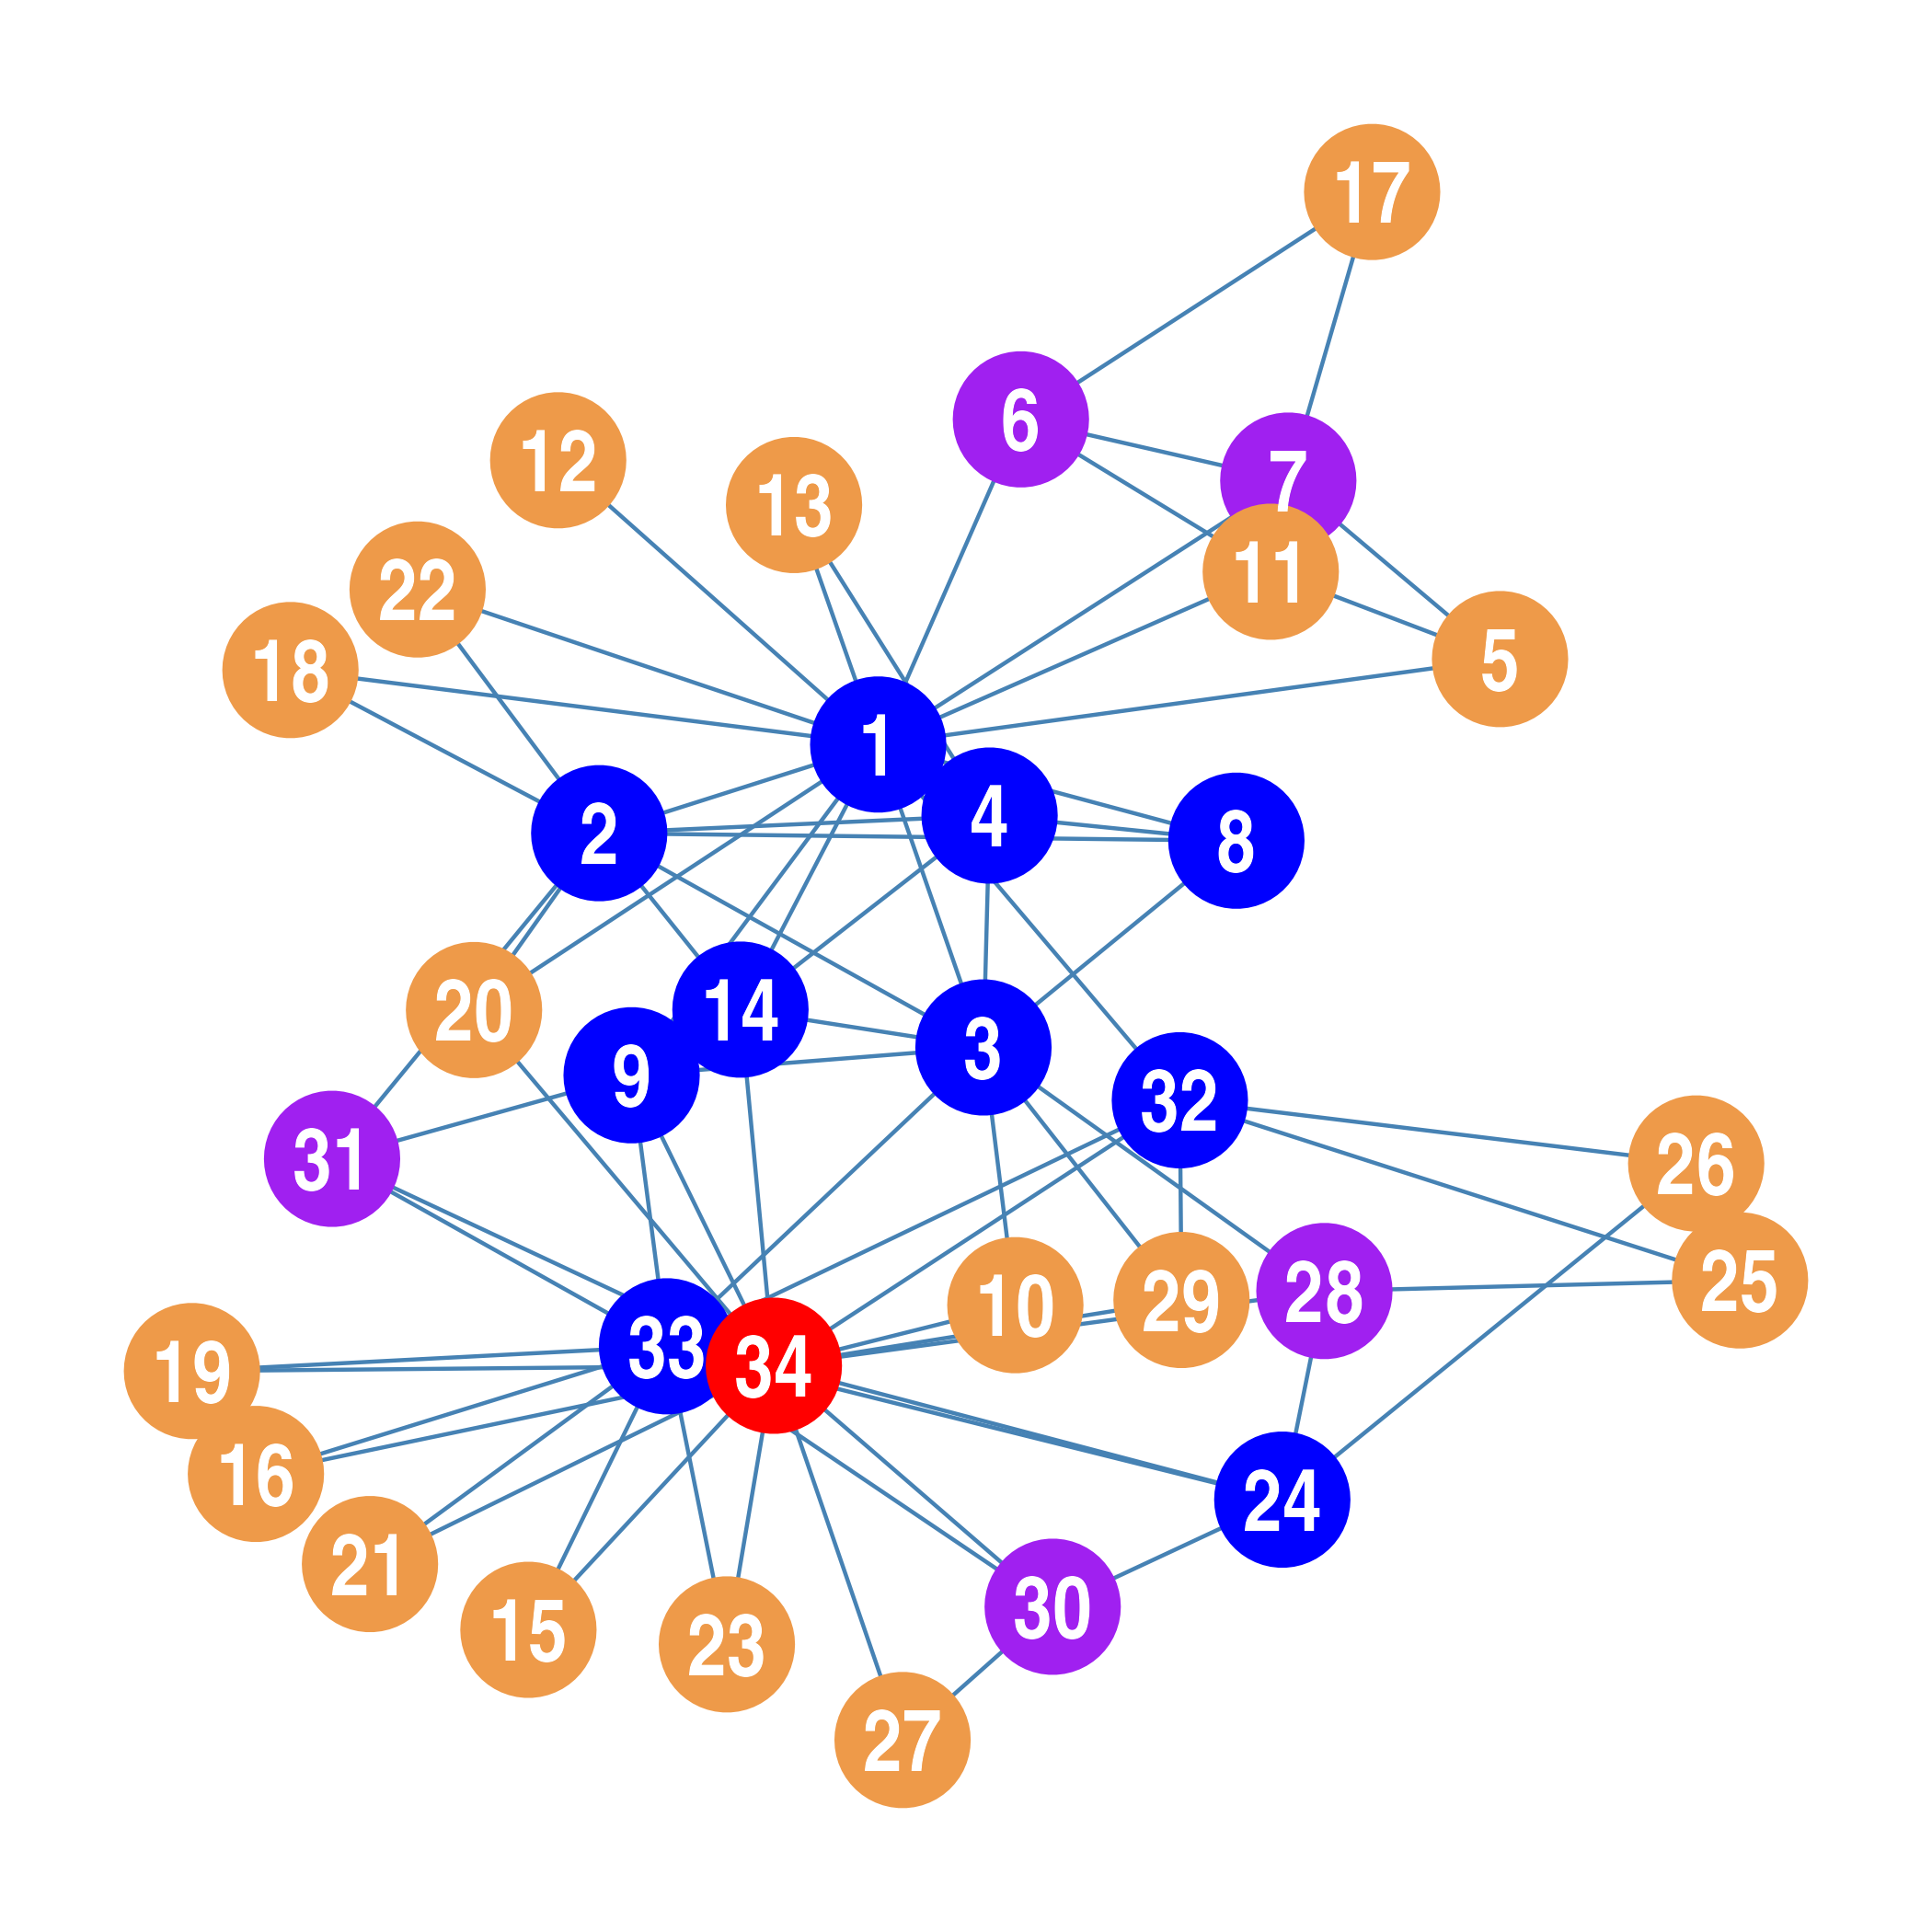
\includegraphics[width=1.0\textwidth]{Plots/kite.png}
            \caption{Six-Clique}
            \label{fig:six-clique}
    \end{subfigure}
    \begin{subfigure}[b]{0.23\textwidth}
        
\includegraphics[width=1.0\textwidth]{Plots/ten-clique-edge.png}
            \caption{Ten-Clique}
            \label{fig:ten-clique}
    \end{subfigure} 
    \begin{subfigure}[b]{0.23\textwidth}
        
\includegraphics[width=1.0\textwidth]{Plots/wheel-clique.png}
            \caption{Three Levels of Hierarchy}
            \label{fig:three-levels}
    \end{subfigure} 
    \begin{subfigure}[b]{0.23\textwidth}
        
\includegraphics[width=1.0\textwidth]{Plots/wheel-clique-edge-star.png}
            \caption{Kite Connects to Highest Distinction Node}
            \label{fig:kite-star}
    \end{subfigure} 
    \begin{subfigure}[b]{0.23\textwidth}
        
\includegraphics[width=1.0\textwidth]{Plots/wheel-clique-edge-clique.png}
            \caption{Kite Connects to Moderate Distinction Node}
            \label{fig:kite-clique}
    \end{subfigure} 
    \begin{subfigure}[b]{0.23\textwidth}
        
\includegraphics[width=1.0\textwidth]{Plots/wheel-clique-edge-peri.png}
            \caption{Kite Connects to Lowest Distinction Node}
            \label{fig:kite-peri}
    \end{subfigure} 
    \begin{subfigure}[b]{0.23\textwidth}
        
\includegraphics[width=1.0\textwidth]{Plots/regular-four.png}
            \caption{Kite Connects to Moderate Distinction Node}
            \label{fig:kite-mod}
    \end{subfigure} 
    \begin{subfigure}[b]{0.23\textwidth}
        
\includegraphics[width=1.0\textwidth]{Plots/regular-edge.png}
            \caption{Kite Connects to Lowest Distinction Node}
            \label{fig:kite-low}
    \end{subfigure} 
    \begin{subfigure}[b]{0.23\textwidth}
        
\includegraphics[width=1.0\textwidth]{Plots/small-world.png}
            \caption{Small World}
            \label{fig:kite-sw}
    \end{subfigure} 
    \begin{subfigure}[b]{0.23\textwidth}
        
\includegraphics[width=1.0\textwidth]{Plots/small-world-edge.png}
            \caption{Small World Kite}
            \label{fig:kite-sw-edge}
    \end{subfigure} 
    \caption{Comparison of kite graphs with varying parameters. Distinction Centrality in toy graphs. Nodes with the highest distinction are shown in red, nodes with positive distinction are shown in blue, nodes with negative distinction are shown in tan, and nodes with distinction close to zero are shown in purple.}
\end{figure}


     \begin{subfigure}[b]{0.3\textwidth}
        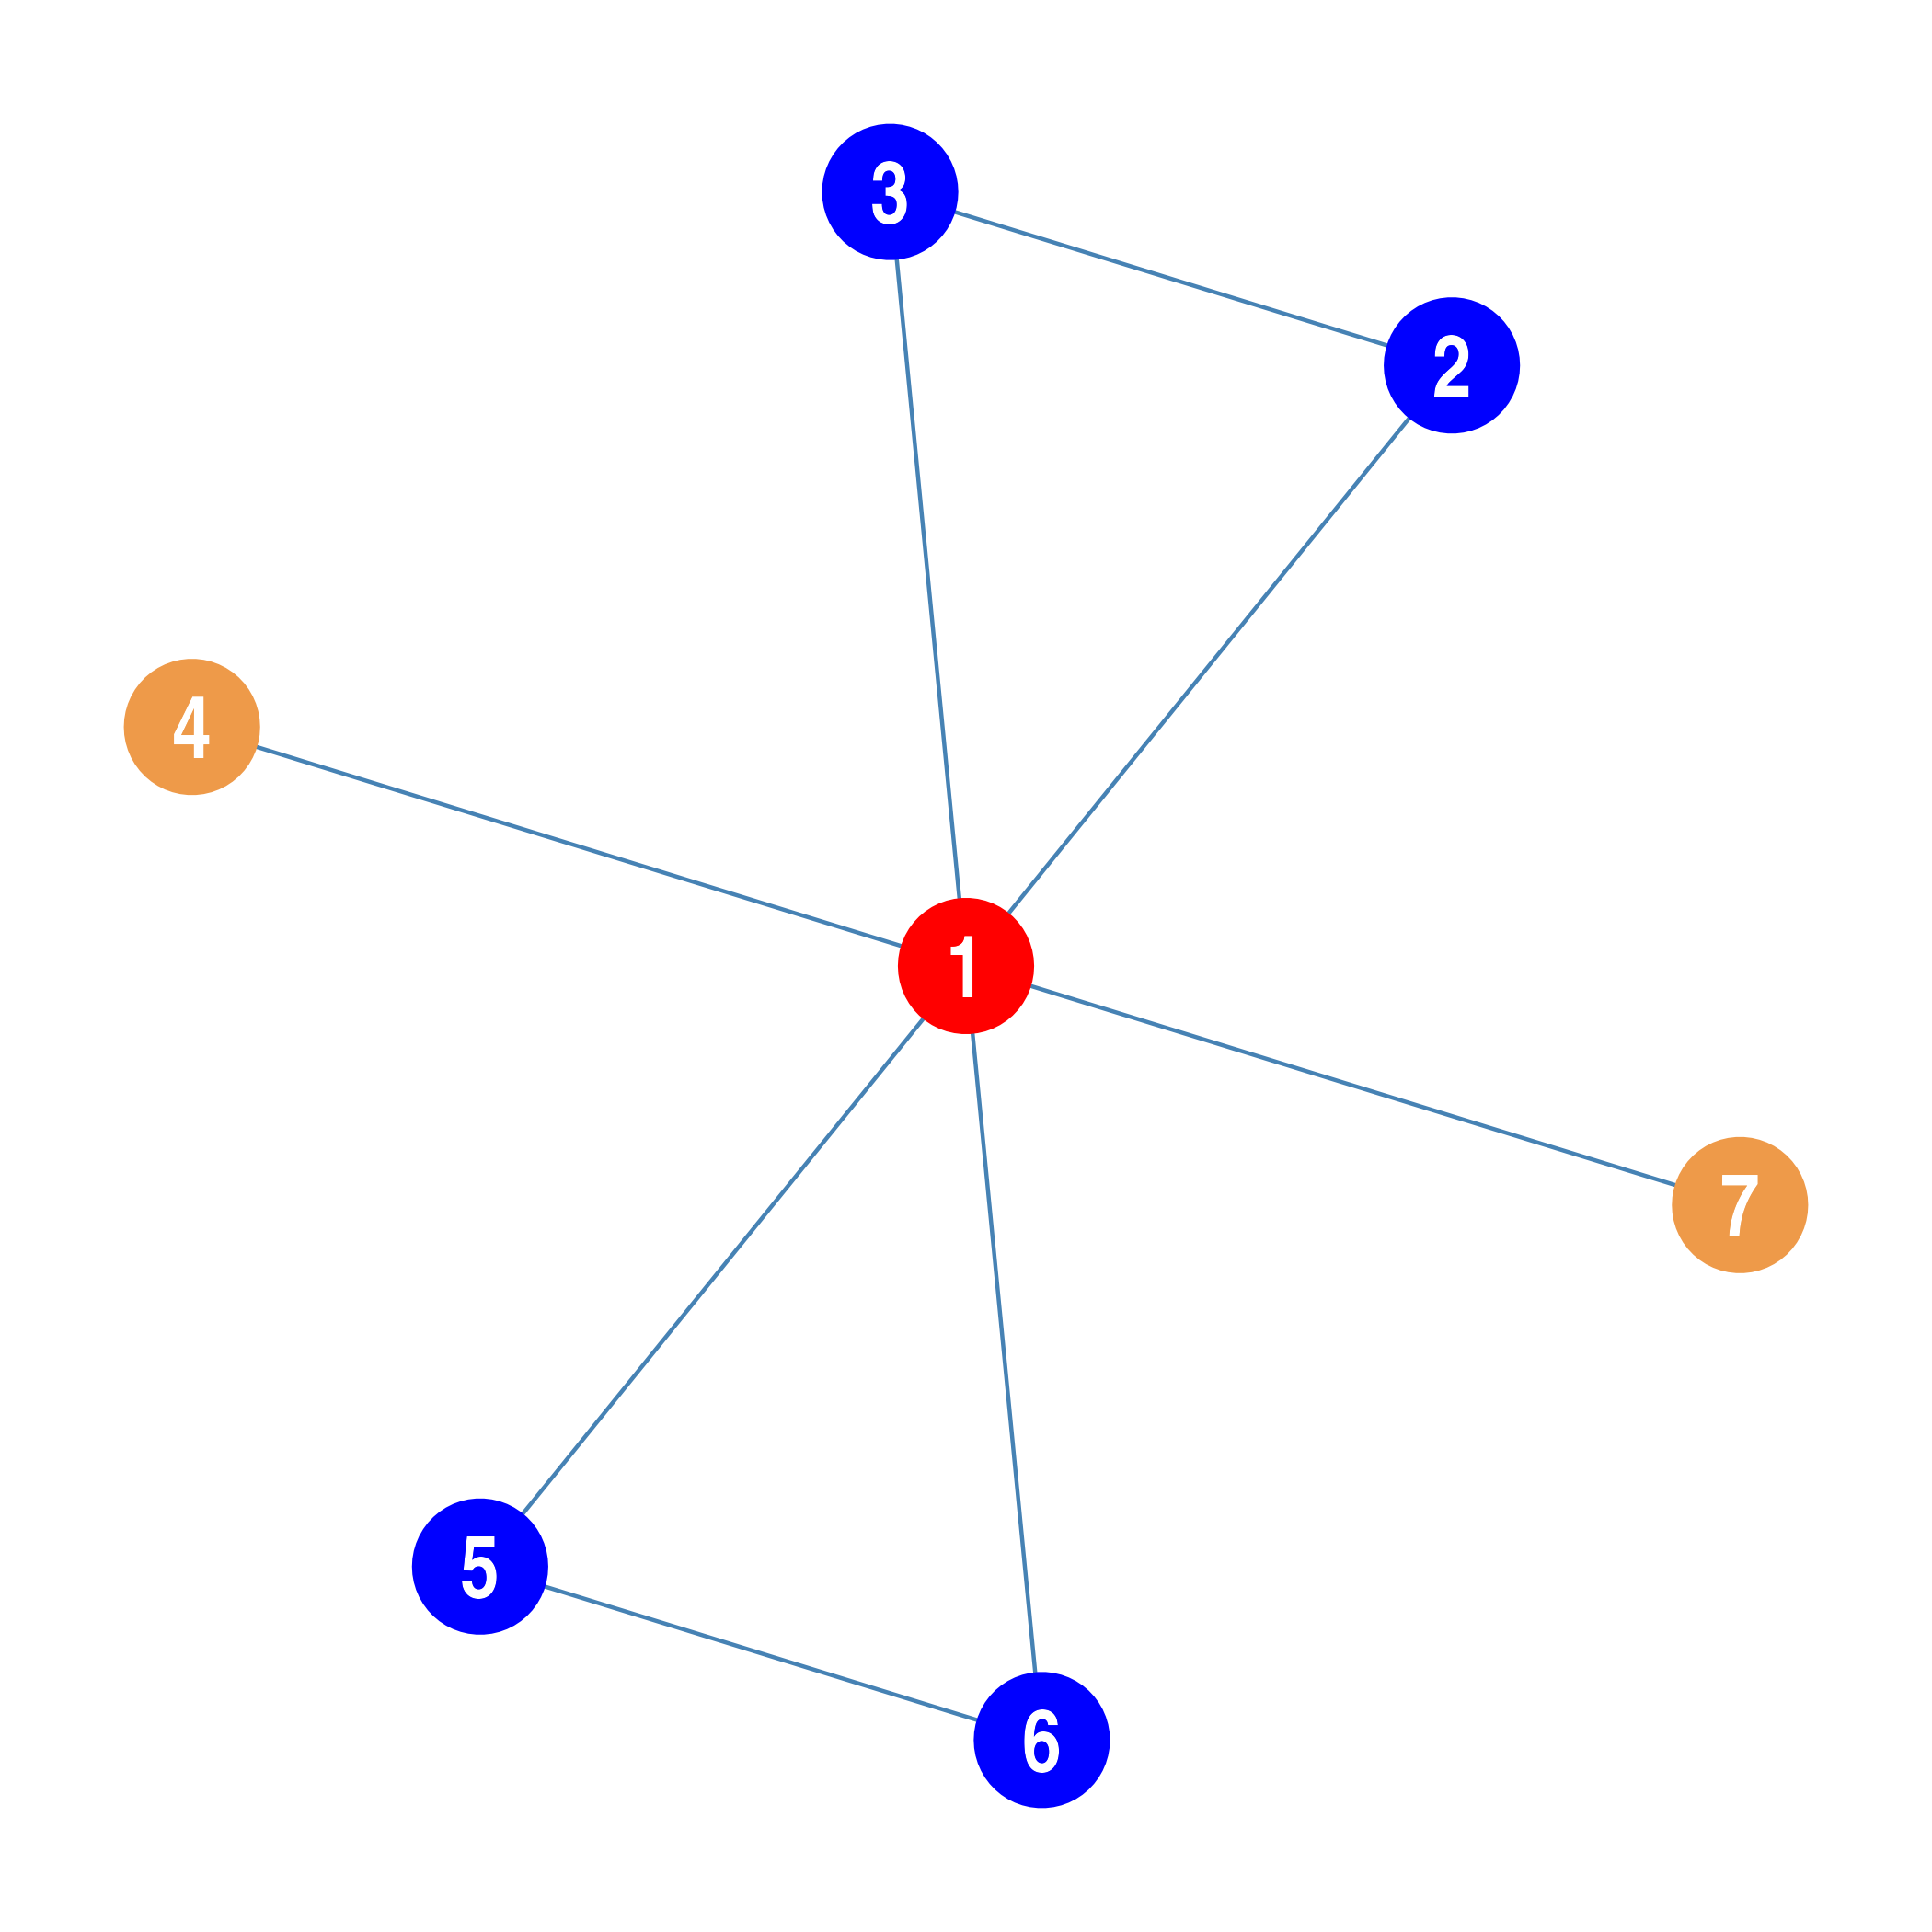
\includegraphics[width=1.0\textwidth]{Plots/star-triangle2.png}
            \caption{Star Graph with Two Triangles}
            \label{fig:startriangle2}
    \end{subfigure}
     \begin{subfigure}[b]{0.3\textwidth}
        
\includegraphics[width=1.0\textwidth]{Plots/two-connected-long.png}
            \caption{2-Connected Subgraphs with Long Tie}
            \label{fig:twoconnectedlong}
    \end{subfigure}



\input{Tabs/Figure5(kites)}



%gets close to 0 negative, with non-normalized eigenvectors
%if you normalize then it all works as expected
% in the normalized kite graph, 1.0, the other get close, decreases the scalar, evs don't mean anything
% computational experiment where you make kite less dense, or size of kite
%kite graph-outsider breaks mechanical solidarity
%mechanical solidarity is really an outcome of the network structure (Durkheim kind of %said that but Omar said it better). Try to get inequality in an organic solidarity system but that's unstable? (might have written that down wrong). 
%mechanical solidarity benefits from the stranger. more theoretical than empirical. 
%actually anthropologists ruined everything in the villages
%also somewhat the Marco Polo vibe, Shogun (the violation of markers of distinction, %didn't matter), The Last Samurai
%theory of subgraph cliques rather than full graph as clique
%hypothesis: size of the normalization gaps is causing the differences between normalized and unnormalized. 

\subsubsection{Long Ties and Hierarchy}

%Strogatz is random, preferential attachment of closure
%Status homophilous (enh) attachment vs preferential vs random 
%*Tie that cuts the longest shortest path Science, 
%https://www.science.org/doi/full/10.1126/science.aau9735
%Distinction homophily, chicken or egg of

This section highlights how the hierarchy emerges from redundant connections among the subgraphs. While a star graph clearly creates a hierarchy, adding weight to the broker's alters can flip the hierarchy, particularly when they form denser subgraphs. This is in keeping with the observed structural holes above. 

Graph (b) is the same as graph (a), except that Nodes 12, 13, and 14 are combined into a clique with Node 9. Graph (c) is the same as graph (b) with the addition of Nodes 21, 22, and 23 as personal connections of Nodes 12, 13, and 14. Finally, graph (d) is the same as graph (c), with the addition of three long ties across subgraphs connecting only Nodes 17 and 23 and 11 and 18.

As Figure 5 graph (d) demonstrates, when those subgroups become redundantly connected not through the central figure but through the sparse interconnections among the other members, Node 9's position of distinction becomes highly elevated.

Thus, there is a U-shaped pattern in which, at low levels of interconnection among sparse subgroups mediated by a central node, the broker's distinction level is high. However, as those subgraphs become more densely connected, the central node's position weakens as status accrues more heavily within those local subgraphs. However, when sparse long connections form between the subgraphs, Node 9 again achieves a high level of distinction because the overall constraint in the network increases with the added ties between the subgraphs. The resulting decrease in the scalar works to stratify the distinction distance between Node 9 and other high-status competitors, while simultaneously decreasing the constraint forced upon Node 9 

\begin{figure}
    \captionsetup[subfigure]{font=footnotesize,labelfont=footnotesize}
    \centering
    \begin{subfigure}[b]{0.9\textwidth}
        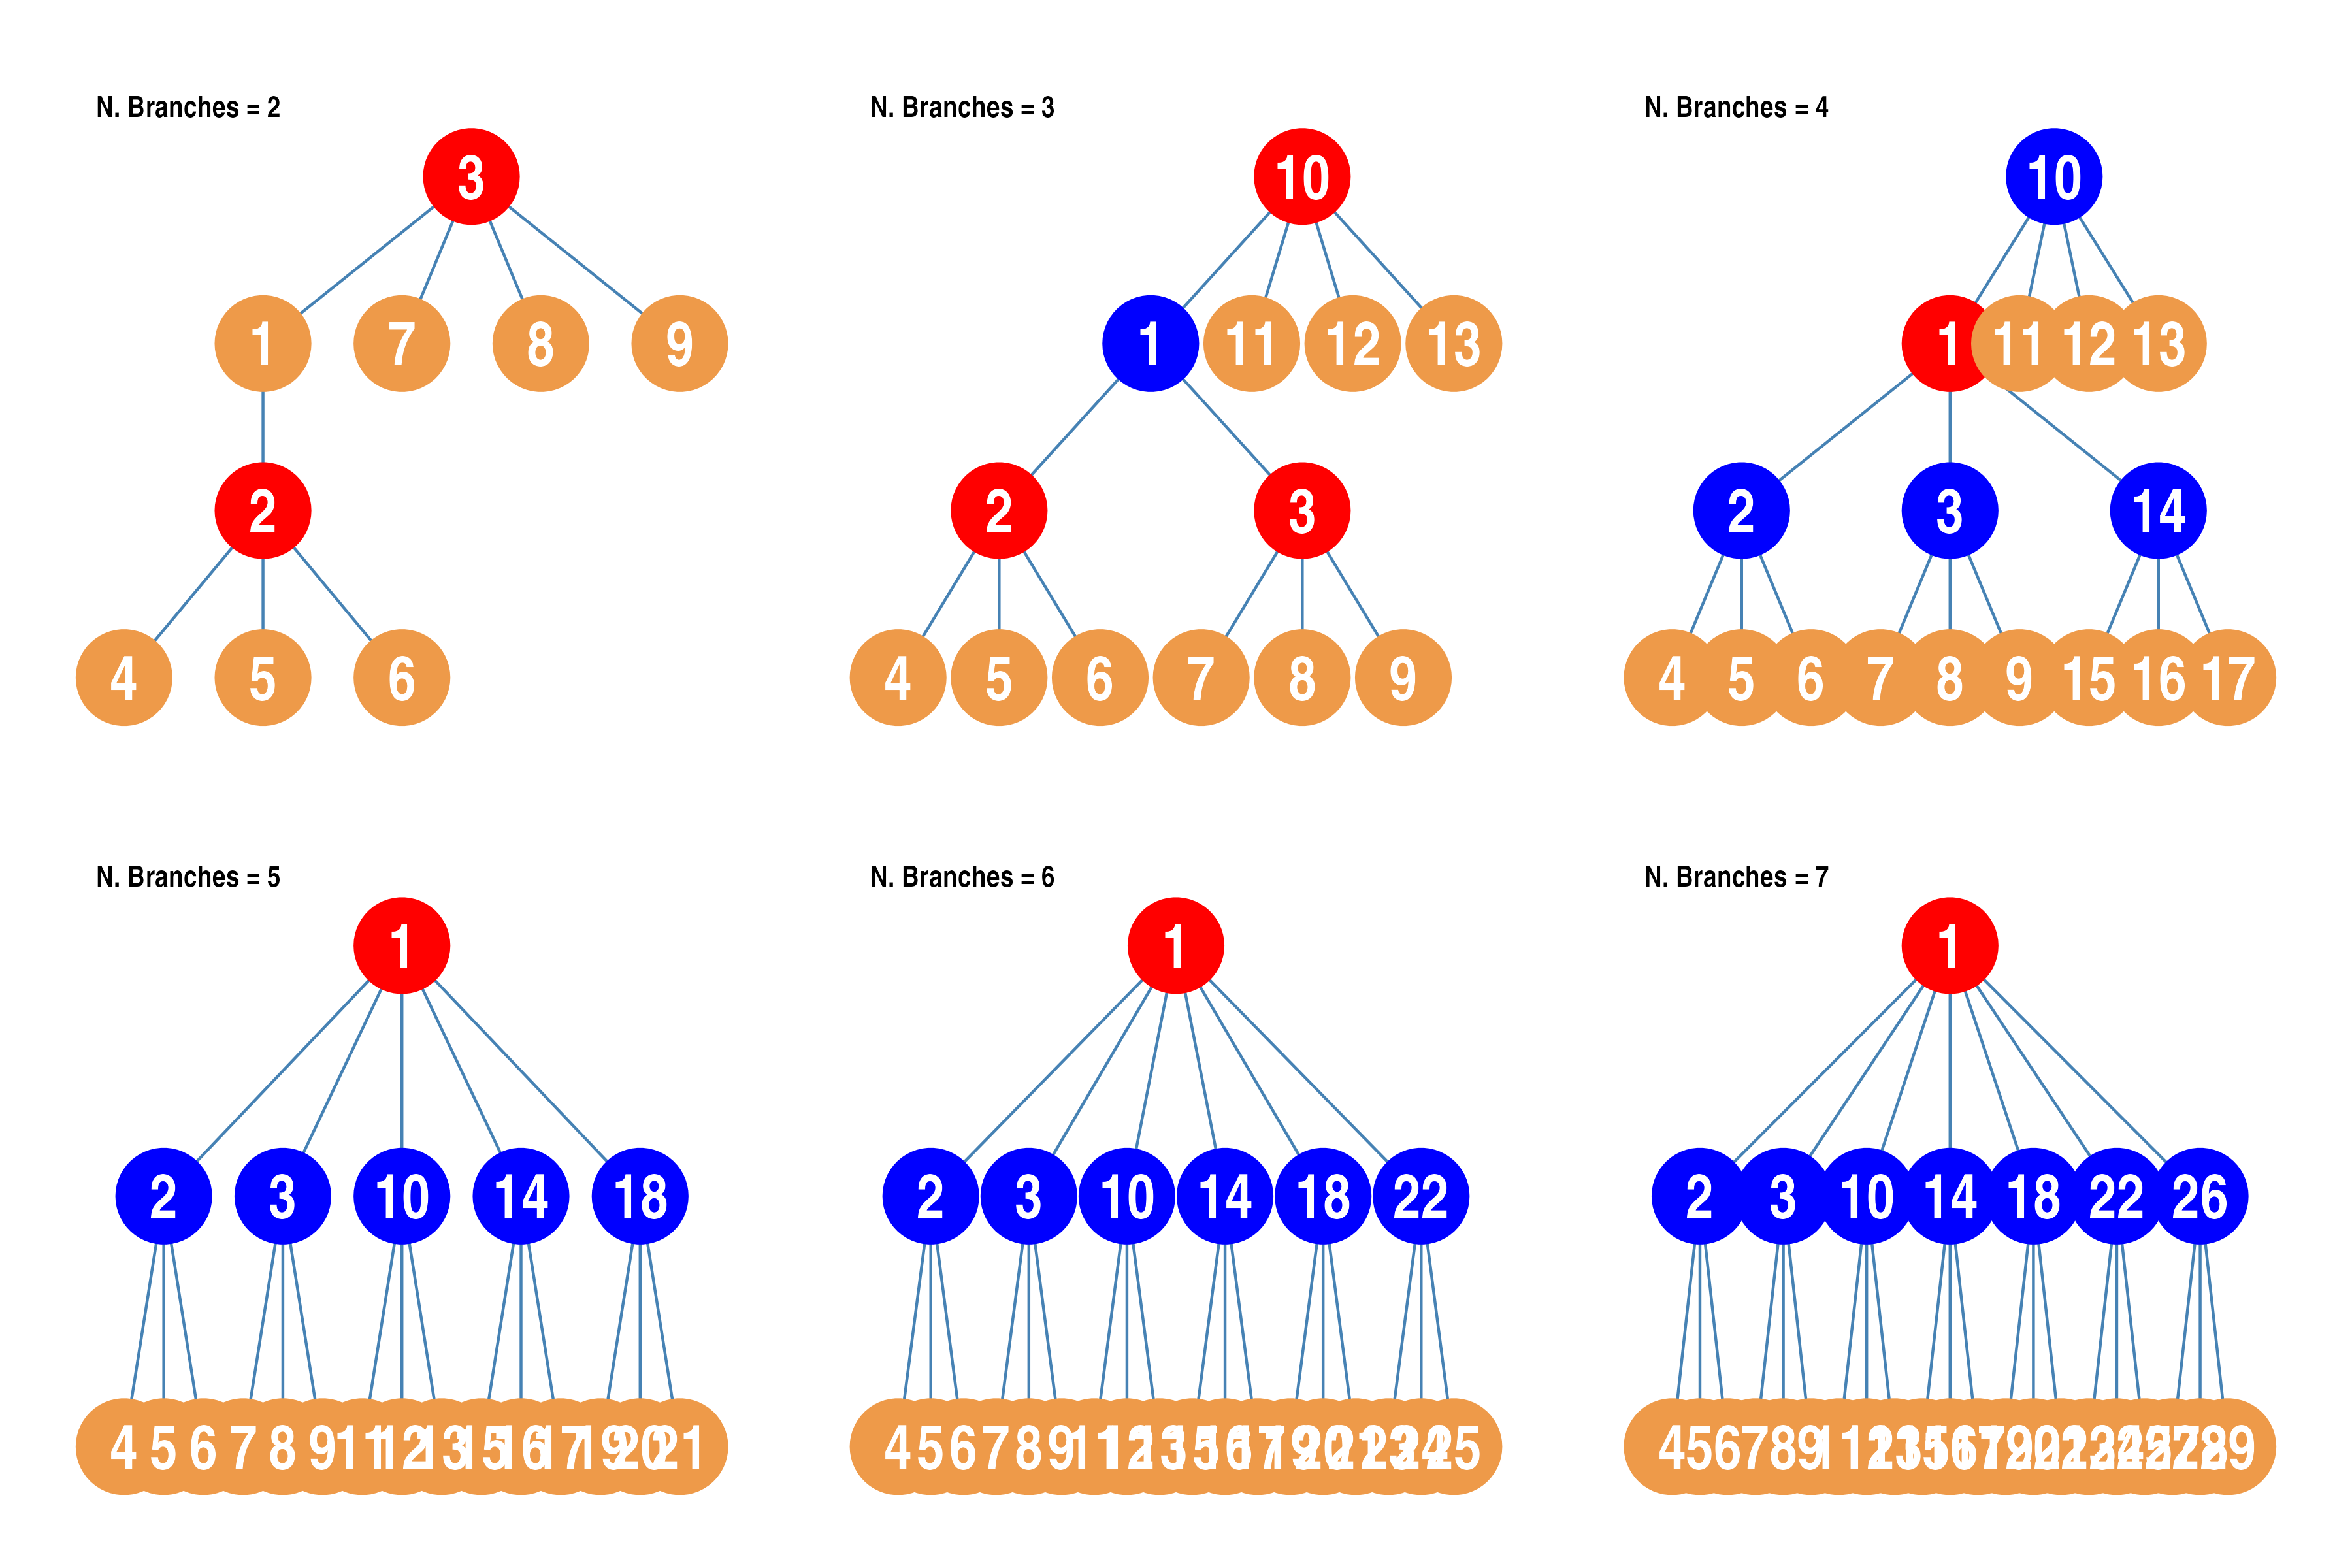
\includegraphics[width=1.0\textwidth]{Plots/tree-examples.png}
            \caption{Example of tree graphs with different numbers of branches for the star node.}
            \label{fig:tree-examples}
    \end{subfigure} \\
    \begin{subfigure}[b]{0.55\textwidth}
        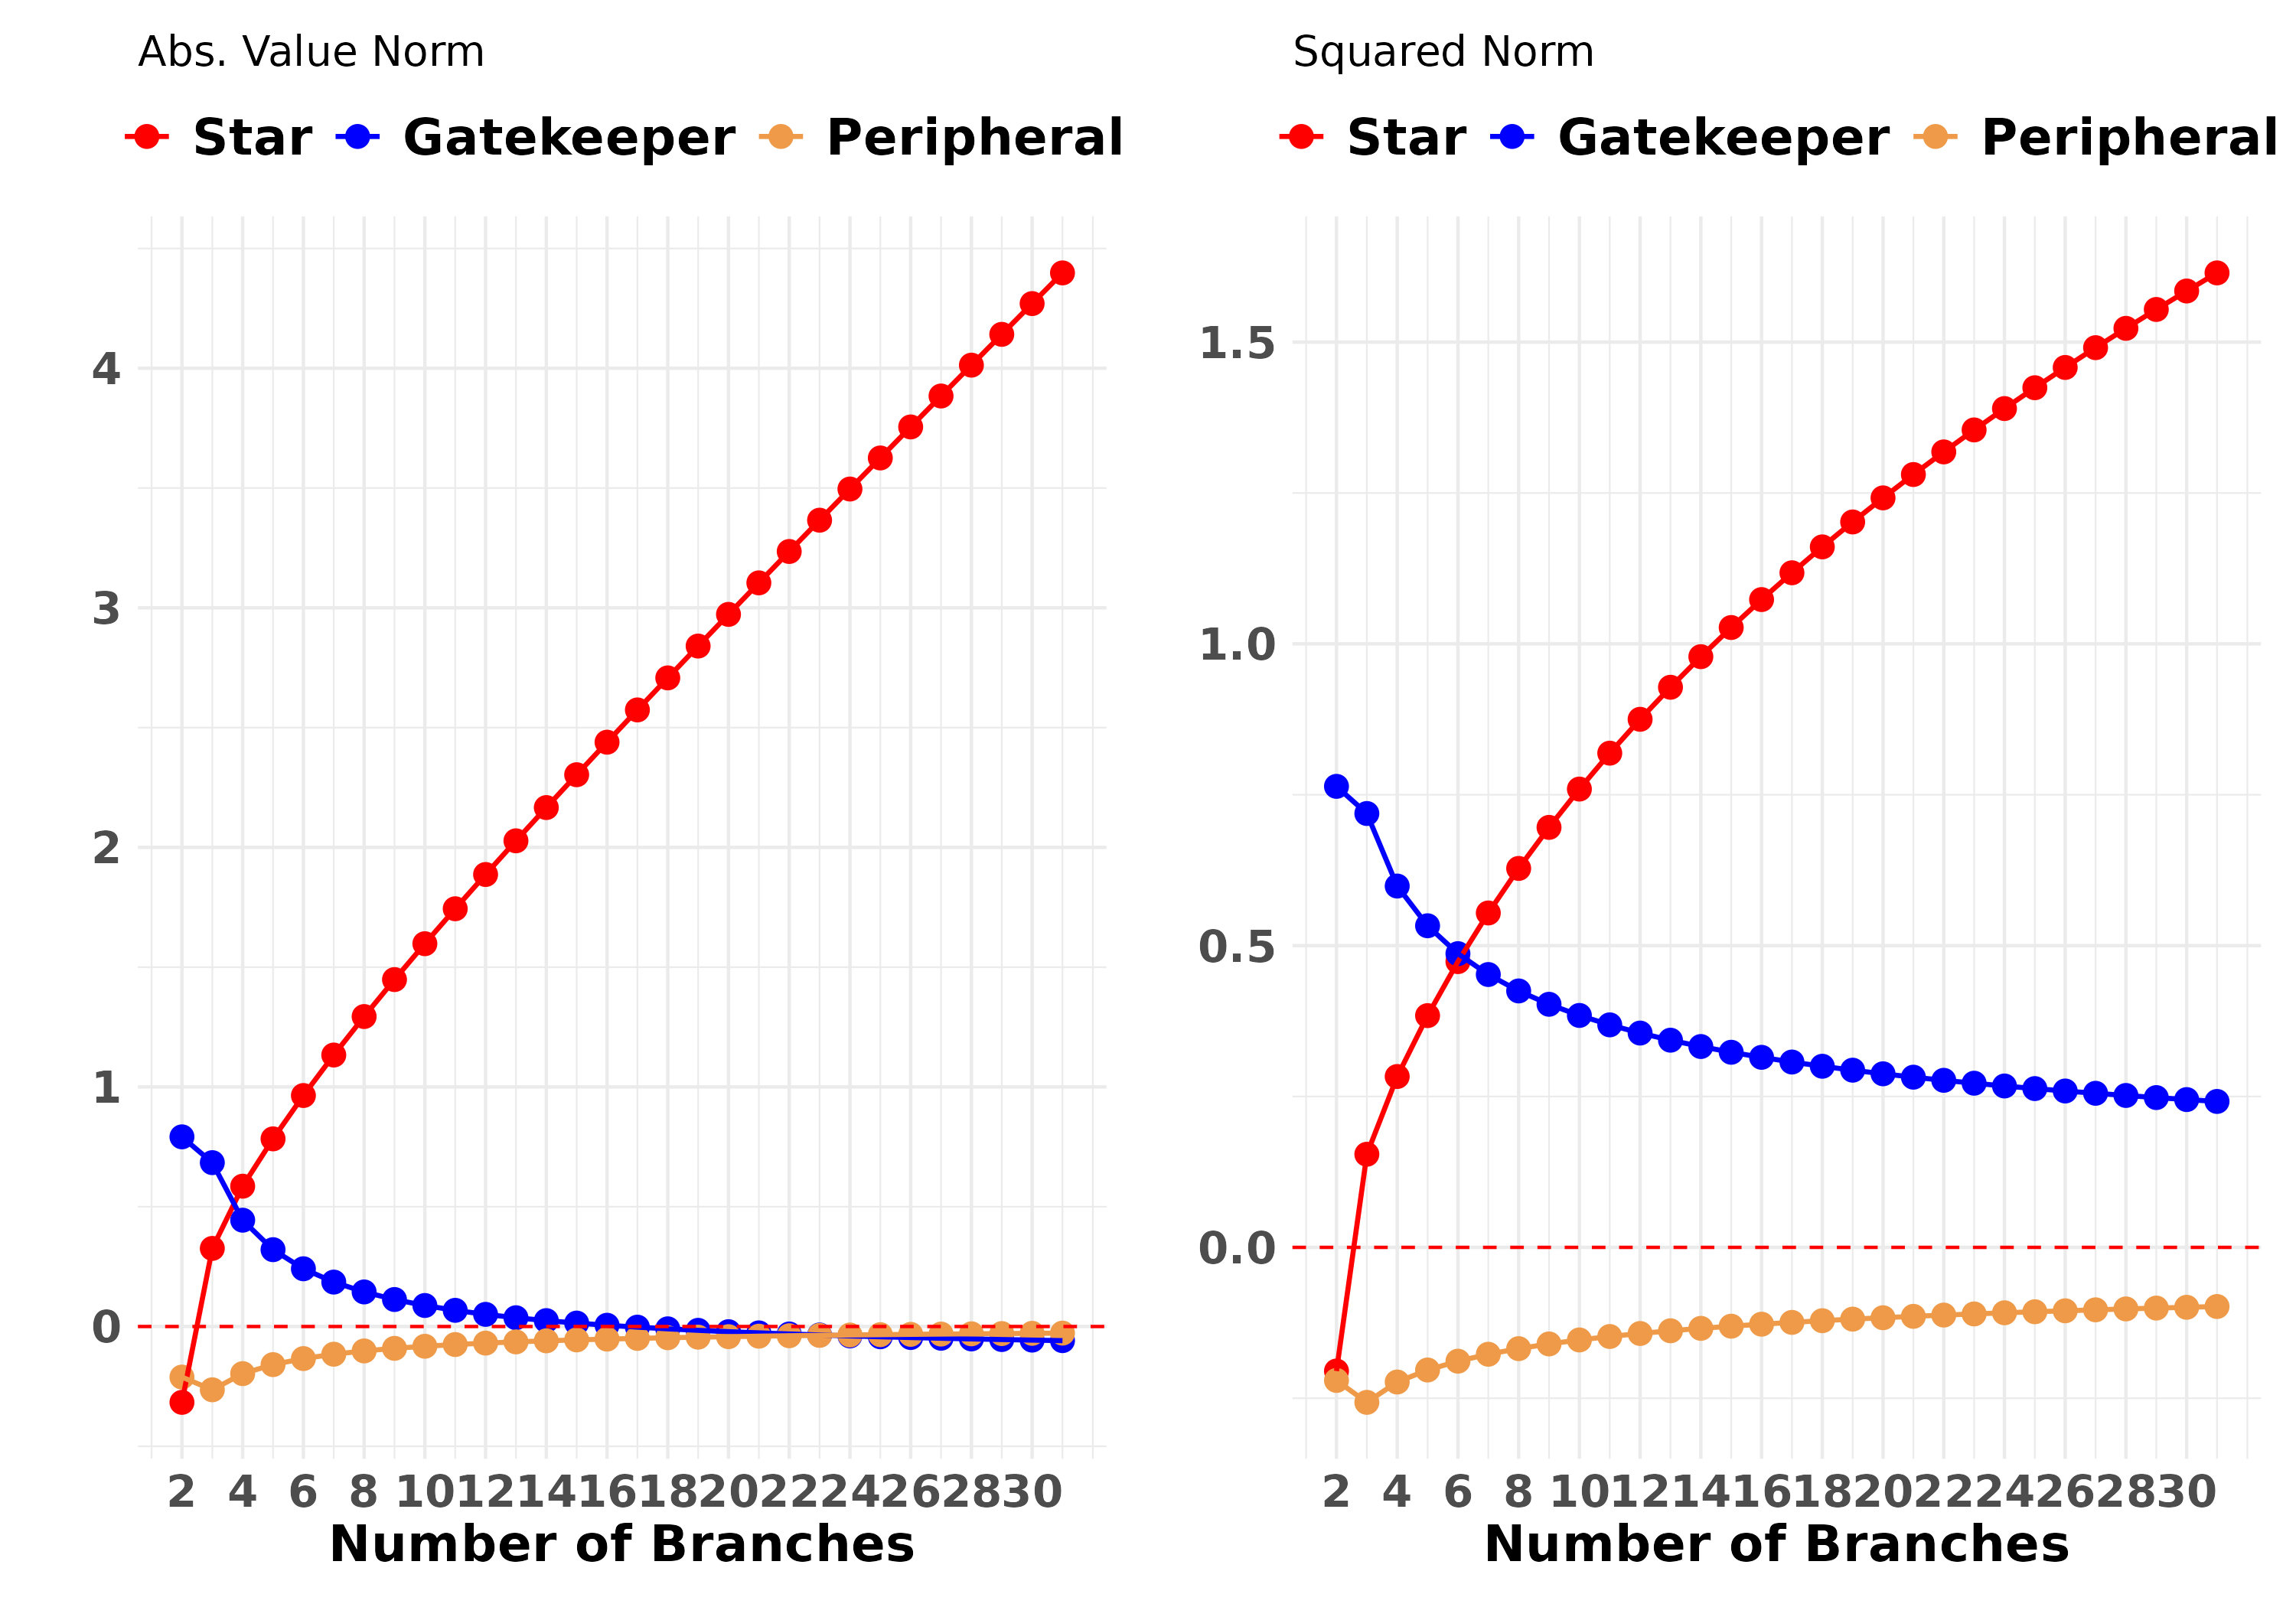
\includegraphics[width=1.0\textwidth]{Plots/broker-tree-roles-by-nbranches.png}
            \caption{Evolution of distinction scores by number of branches for the star node.}
            \label{fig:broker-tree-roles}
    \end{subfigure}
    \caption{.}
    \label{fig:toys}
\end{figure}


\begin{figure}
    \captionsetup[subfigure]{font=footnotesize,labelfont=footnotesize}
    \centering
     \begin{subfigure}[b]{0.45\textwidth}
        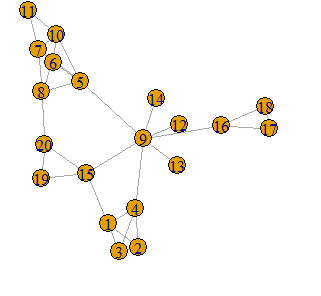
\includegraphics[width=1.0\textwidth]{Plots/political1.png}
            \caption{High Subgraph Density, Low Graph Density}
            \label{fig:pol1}
    \end{subfigure}
     \begin{subfigure}[b]{0.45\textwidth}
        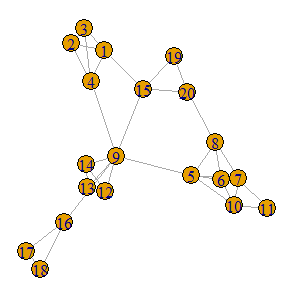
\includegraphics[width=1.0\textwidth]{Plots/political2.png}
            \caption{Broker Given Independent Foundations}
            \label{fig:pol2}
    \end{subfigure}
         \begin{subfigure}[b]{0.45\textwidth}
        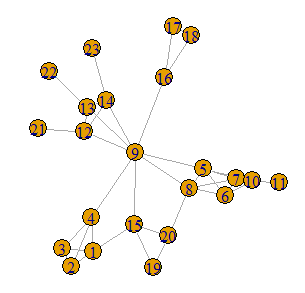
\includegraphics[width=1.0\textwidth]{Plots/political3.png}
            \caption{Increased Independent Foundations}
            \label{fig:pol3}
    \end{subfigure}
     \begin{subfigure}[b]{0.45\textwidth}
        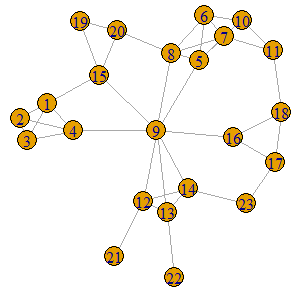
\includegraphics[width=1.0\textwidth]{Plots/political4.png}
            \caption{All Subgraphs Connected by Long Ties}
            \label{fig:pol4}
    \end{subfigure}
    \caption{Increasingly connected graphs with central broker.}
    \label{fig:Evolving Political Network}
\end{figure}

\input{Tabs/Figure6.tex}


\begin{figure}
    \captionsetup[subfigure]{font=footnotesize,labelfont=footnotesize}
    \centering
    \begin{subfigure}[b]{0.36\textwidth}
        
\includegraphics[width=1.0\textwidth]{Plots/regular-four.png}
            \caption{Regular graph of degree four.}
            \label{fig:reg4}
    \end{subfigure} 
    \begin{subfigure}[b]{0.36\textwidth}
        
\includegraphics[width=1.0\textwidth]{Plots/small-world1.png}
            \caption{SW network with one long tie.}
            \label{fig:sw1-1}
    \end{subfigure} \\
    \begin{subfigure}[b]{0.36\textwidth}
        
\includegraphics[width=1.0\textwidth]{Plots/small-world2.png}
            \caption{SW network with two long ties.}
            \label{fig:sw1-2}
    \end{subfigure}
    \begin{subfigure}[b]{0.36\textwidth}
        
\includegraphics[width=1.0\textwidth]{Plots/small-world3.png}
            \caption{SW network with three long ties.}
            \label{fig:sw1-3}
    \end{subfigure}
    \caption{.}
\end{figure}